% Options for packages loaded elsewhere
\PassOptionsToPackage{unicode}{hyperref}
\PassOptionsToPackage{hyphens}{url}
\PassOptionsToPackage{dvipsnames,svgnames,x11names}{xcolor}
%
\documentclass[
  letterpaper,
  DIV=11,
  numbers=noendperiod]{scrartcl}

\usepackage{amsmath,amssymb}
\usepackage{iftex}
\ifPDFTeX
  \usepackage[T1]{fontenc}
  \usepackage[utf8]{inputenc}
  \usepackage{textcomp} % provide euro and other symbols
\else % if luatex or xetex
  \usepackage{unicode-math}
  \defaultfontfeatures{Scale=MatchLowercase}
  \defaultfontfeatures[\rmfamily]{Ligatures=TeX,Scale=1}
\fi
\usepackage{lmodern}
\ifPDFTeX\else  
    % xetex/luatex font selection
\fi
% Use upquote if available, for straight quotes in verbatim environments
\IfFileExists{upquote.sty}{\usepackage{upquote}}{}
\IfFileExists{microtype.sty}{% use microtype if available
  \usepackage[]{microtype}
  \UseMicrotypeSet[protrusion]{basicmath} % disable protrusion for tt fonts
}{}
\makeatletter
\@ifundefined{KOMAClassName}{% if non-KOMA class
  \IfFileExists{parskip.sty}{%
    \usepackage{parskip}
  }{% else
    \setlength{\parindent}{0pt}
    \setlength{\parskip}{6pt plus 2pt minus 1pt}}
}{% if KOMA class
  \KOMAoptions{parskip=half}}
\makeatother
\usepackage{xcolor}
\setlength{\emergencystretch}{3em} % prevent overfull lines
\setcounter{secnumdepth}{5}
% Make \paragraph and \subparagraph free-standing
\makeatletter
\ifx\paragraph\undefined\else
  \let\oldparagraph\paragraph
  \renewcommand{\paragraph}{
    \@ifstar
      \xxxParagraphStar
      \xxxParagraphNoStar
  }
  \newcommand{\xxxParagraphStar}[1]{\oldparagraph*{#1}\mbox{}}
  \newcommand{\xxxParagraphNoStar}[1]{\oldparagraph{#1}\mbox{}}
\fi
\ifx\subparagraph\undefined\else
  \let\oldsubparagraph\subparagraph
  \renewcommand{\subparagraph}{
    \@ifstar
      \xxxSubParagraphStar
      \xxxSubParagraphNoStar
  }
  \newcommand{\xxxSubParagraphStar}[1]{\oldsubparagraph*{#1}\mbox{}}
  \newcommand{\xxxSubParagraphNoStar}[1]{\oldsubparagraph{#1}\mbox{}}
\fi
\makeatother


\providecommand{\tightlist}{%
  \setlength{\itemsep}{0pt}\setlength{\parskip}{0pt}}\usepackage{longtable,booktabs,array}
\usepackage{calc} % for calculating minipage widths
% Correct order of tables after \paragraph or \subparagraph
\usepackage{etoolbox}
\makeatletter
\patchcmd\longtable{\par}{\if@noskipsec\mbox{}\fi\par}{}{}
\makeatother
% Allow footnotes in longtable head/foot
\IfFileExists{footnotehyper.sty}{\usepackage{footnotehyper}}{\usepackage{footnote}}
\makesavenoteenv{longtable}
\usepackage{graphicx}
\makeatletter
\def\maxwidth{\ifdim\Gin@nat@width>\linewidth\linewidth\else\Gin@nat@width\fi}
\def\maxheight{\ifdim\Gin@nat@height>\textheight\textheight\else\Gin@nat@height\fi}
\makeatother
% Scale images if necessary, so that they will not overflow the page
% margins by default, and it is still possible to overwrite the defaults
% using explicit options in \includegraphics[width, height, ...]{}
\setkeys{Gin}{width=\maxwidth,height=\maxheight,keepaspectratio}
% Set default figure placement to htbp
\makeatletter
\def\fps@figure{htbp}
\makeatother

\KOMAoption{captions}{tableheading}
\makeatletter
\@ifpackageloaded{caption}{}{\usepackage{caption}}
\AtBeginDocument{%
\ifdefined\contentsname
  \renewcommand*\contentsname{Table of contents}
\else
  \newcommand\contentsname{Table of contents}
\fi
\ifdefined\listfigurename
  \renewcommand*\listfigurename{List of Figures}
\else
  \newcommand\listfigurename{List of Figures}
\fi
\ifdefined\listtablename
  \renewcommand*\listtablename{List of Tables}
\else
  \newcommand\listtablename{List of Tables}
\fi
\ifdefined\figurename
  \renewcommand*\figurename{Figure}
\else
  \newcommand\figurename{Figure}
\fi
\ifdefined\tablename
  \renewcommand*\tablename{Table}
\else
  \newcommand\tablename{Table}
\fi
}
\@ifpackageloaded{float}{}{\usepackage{float}}
\floatstyle{ruled}
\@ifundefined{c@chapter}{\newfloat{codelisting}{h}{lop}}{\newfloat{codelisting}{h}{lop}[chapter]}
\floatname{codelisting}{Listing}
\newcommand*\listoflistings{\listof{codelisting}{List of Listings}}
\makeatother
\makeatletter
\makeatother
\makeatletter
\@ifpackageloaded{caption}{}{\usepackage{caption}}
\@ifpackageloaded{subcaption}{}{\usepackage{subcaption}}
\makeatother

\ifLuaTeX
  \usepackage{selnolig}  % disable illegal ligatures
\fi
\usepackage{bookmark}

\IfFileExists{xurl.sty}{\usepackage{xurl}}{} % add URL line breaks if available
\urlstyle{same} % disable monospaced font for URLs
\hypersetup{
  pdftitle={Quantifying comprehensive marine transportation emissions using data fusion},
  pdfauthor={emLab, UCSB and GFW},
  colorlinks=true,
  linkcolor={blue},
  filecolor={Maroon},
  citecolor={Blue},
  urlcolor={Blue},
  pdfcreator={LaTeX via pandoc}}


\title{Quantifying comprehensive marine transportation emissions using
data fusion}
\author{emLab, UCSB and GFW}
\date{Last Updated on June 13, 2025}

\begin{document}
\maketitle

\renewcommand*\contentsname{Table of contents}
{
\hypersetup{linkcolor=}
\setcounter{tocdepth}{3}
\tableofcontents
}

\section{Paper stats}\label{paper-stats}

\subsection{Fraction of total global emissions from the transportation
sector in
2023}\label{fraction-of-total-global-emissions-from-the-transportation-sector-in-2023}

In 2023, the transportation sector contributed 21\% of all CO2 emissions
globally.

\section{Paper figures}\label{paper-figures}

\subsubsection{Figure 1 panel A}\label{figure-1-panel-a}

\begin{longtable}[]{@{}ll@{}}

\caption{\label{tbl-summary-stat-comparison-2023-gfw-edgar}Comparison of
2023 data between marine transportation emissions from GFW and
terrestrial transportation emissions from EDGAR.}

\tabularnewline

\toprule\noalign{}
name & value \\
\midrule\noalign{}
\endhead
\bottomrule\noalign{}
\endlastfoot
emissions\_co2\_billion\_mt\_land\_edgar & 7.3 \\
emissions\_co2\_billion\_mt\_ocean\_gfw & 1.3 \\
emissions\_normalized\_from\_2016\_land\_edgar & 4\% \\
emissions\_normalized\_from\_2016\_ocean\_gfw & 22\% \\
normalized\_ocean\_over\_land & 5.3 \\
fraction\_ocean\_over\_total & 15\% \\

\end{longtable}

\subsubsection{Figure 1}\label{figure-1}

\begin{figure}[H]

\centering{

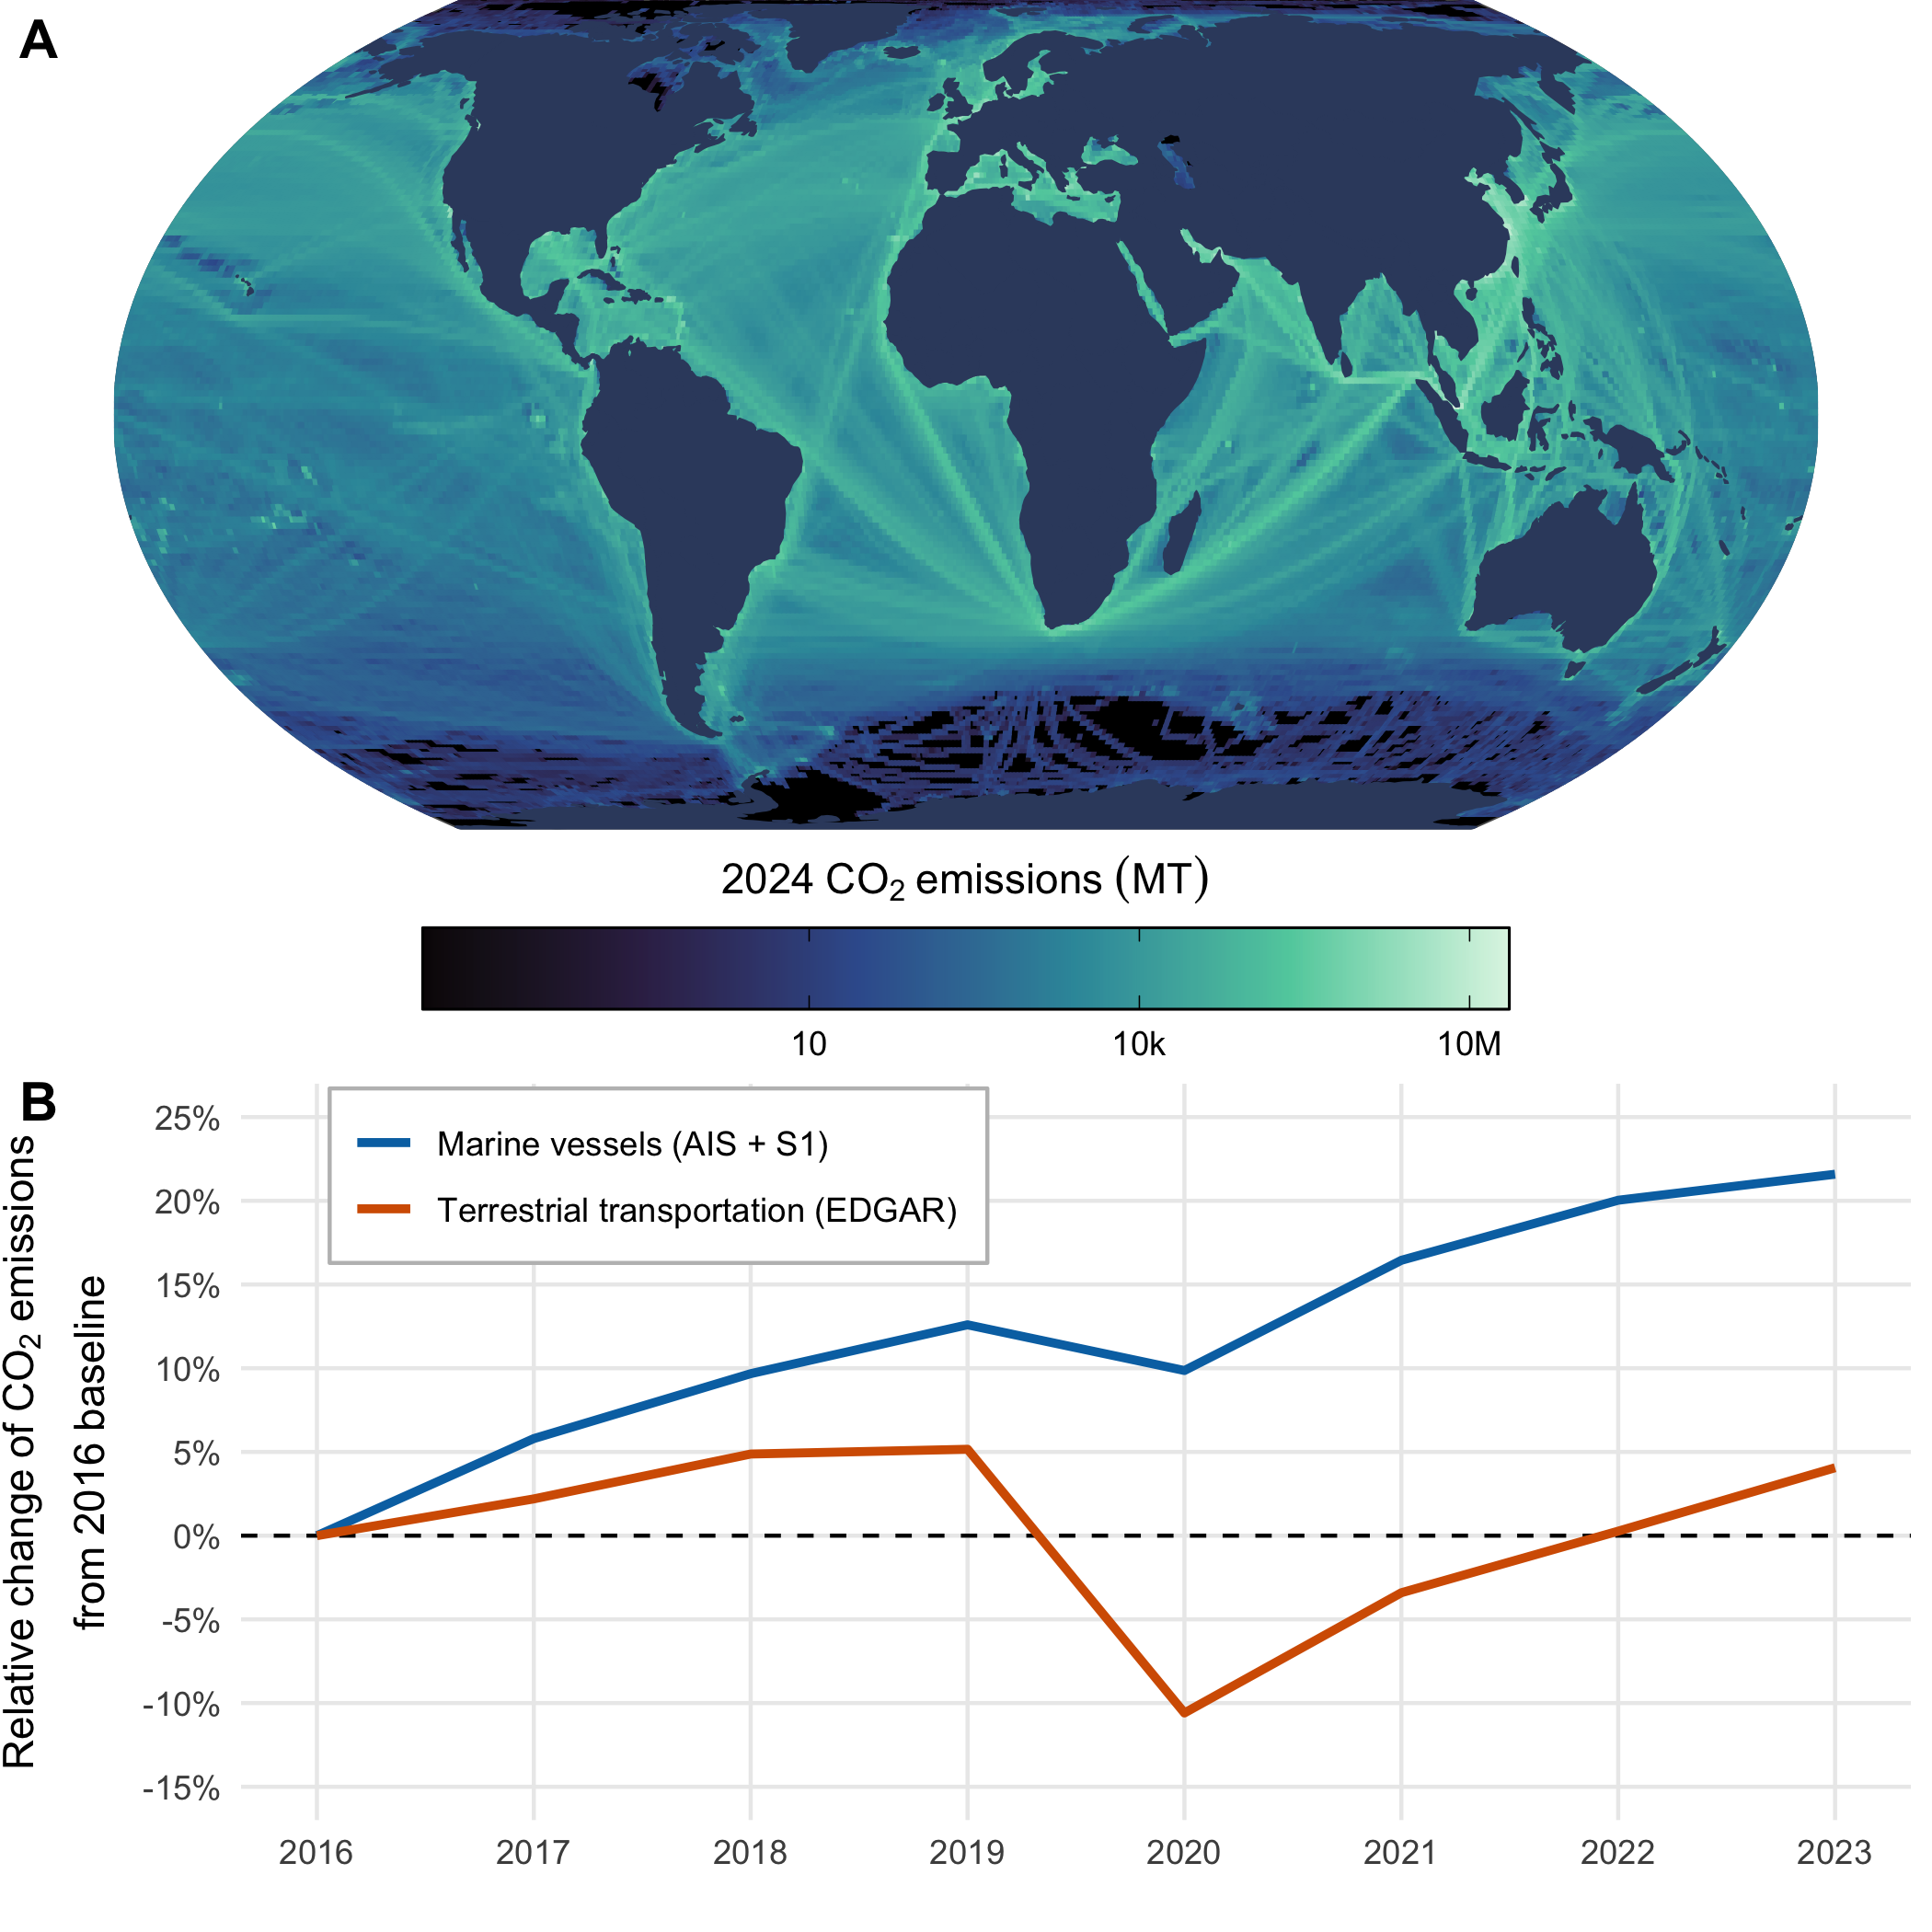
\includegraphics{figures/fig-co2-emissions-map-normalized-sector-time-series-1.png}

}

\caption{\label{fig-co2-emissions-map-normalized-sector-time-series}}

\end{figure}%

\subsubsection{Figure 1 panel A}\label{figure-1-panel-a-1}

\subsection{Figure 1 panel B}\label{figure-1-panel-b}

\subsubsection{Figure 2}\label{figure-2}

\begin{figure}[H]

\centering{


\includegraphics{figures/fig-total-annual-emissions-by-data-source-1.png}

}

\caption{\label{fig-total-annual-emissions-by-data-source}(A) Annual
marine vessel CO2 emissions, with each line colored based on the data
source. (B) Relative change in annual marine vessel CO2 emissions from a
2016 baseline, with each line colored based on the data source.}

\end{figure}%

\section{Supplementary figure - Comparing sector-specific emissions by
data source
(absolute)}\label{supplementary-figure---comparing-sector-specific-emissions-by-data-source-absolute}

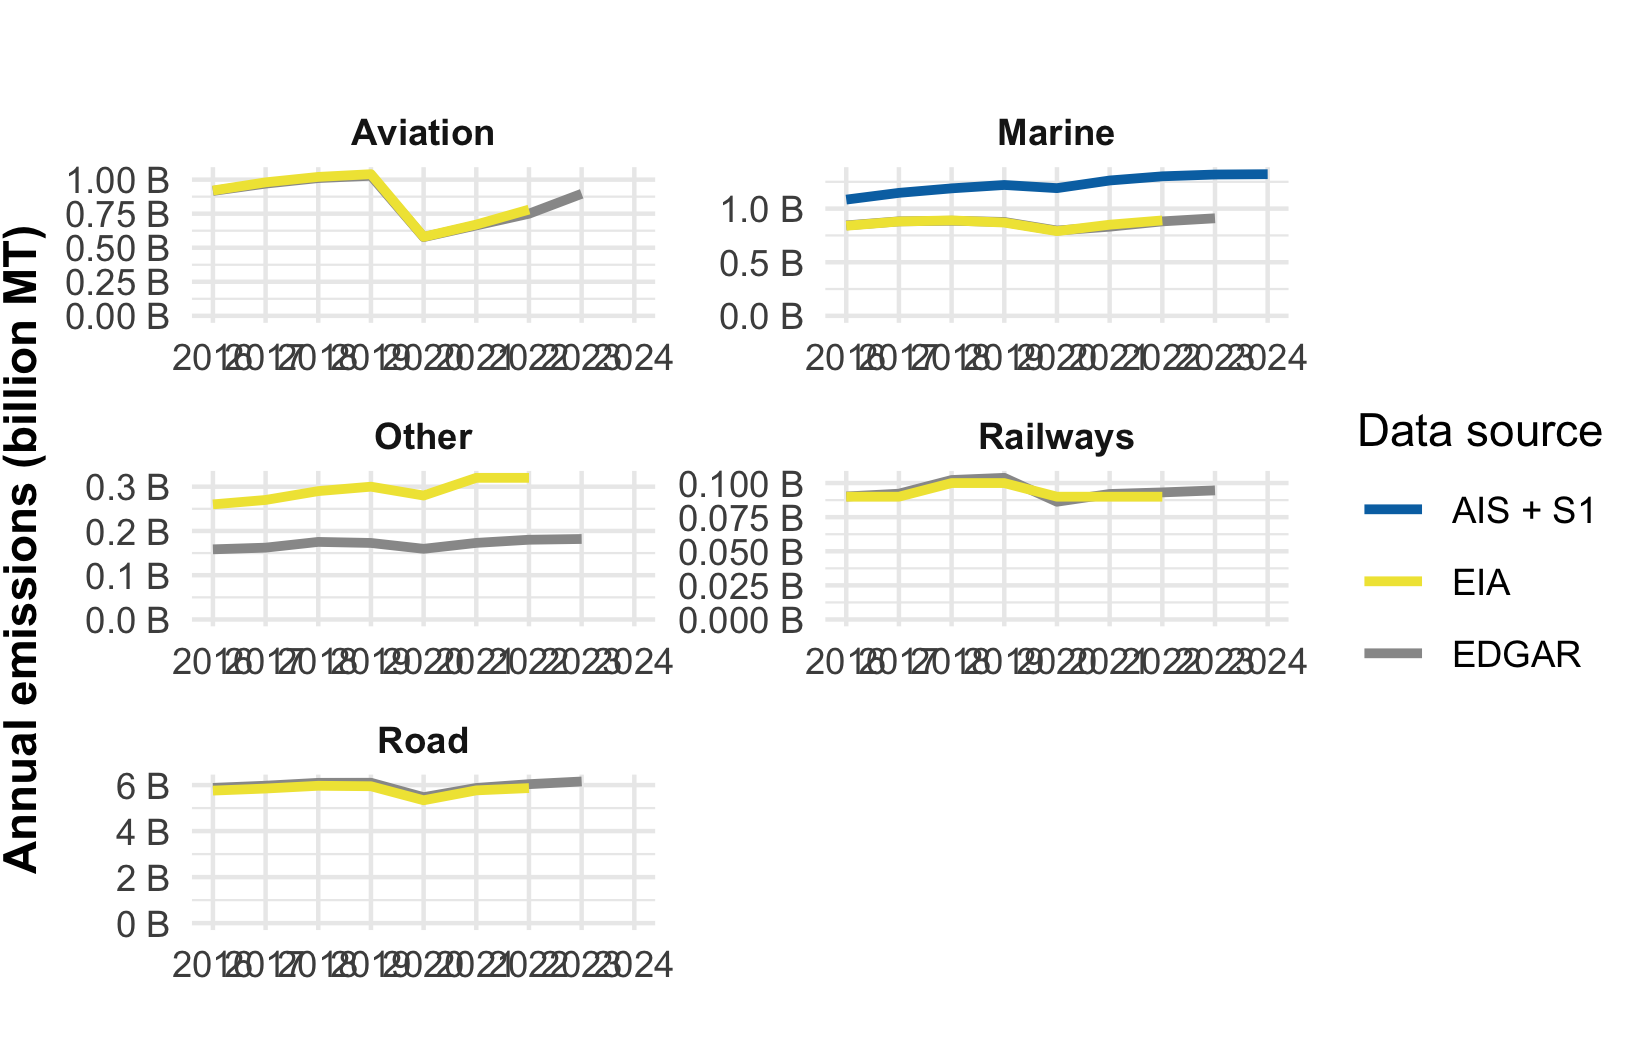
\includegraphics{figures/unnamed-chunk-10-1.png}

\section{Supplementary figure - Comparing sector-specific emissions by
data source
(normalized)}\label{supplementary-figure---comparing-sector-specific-emissions-by-data-source-normalized}

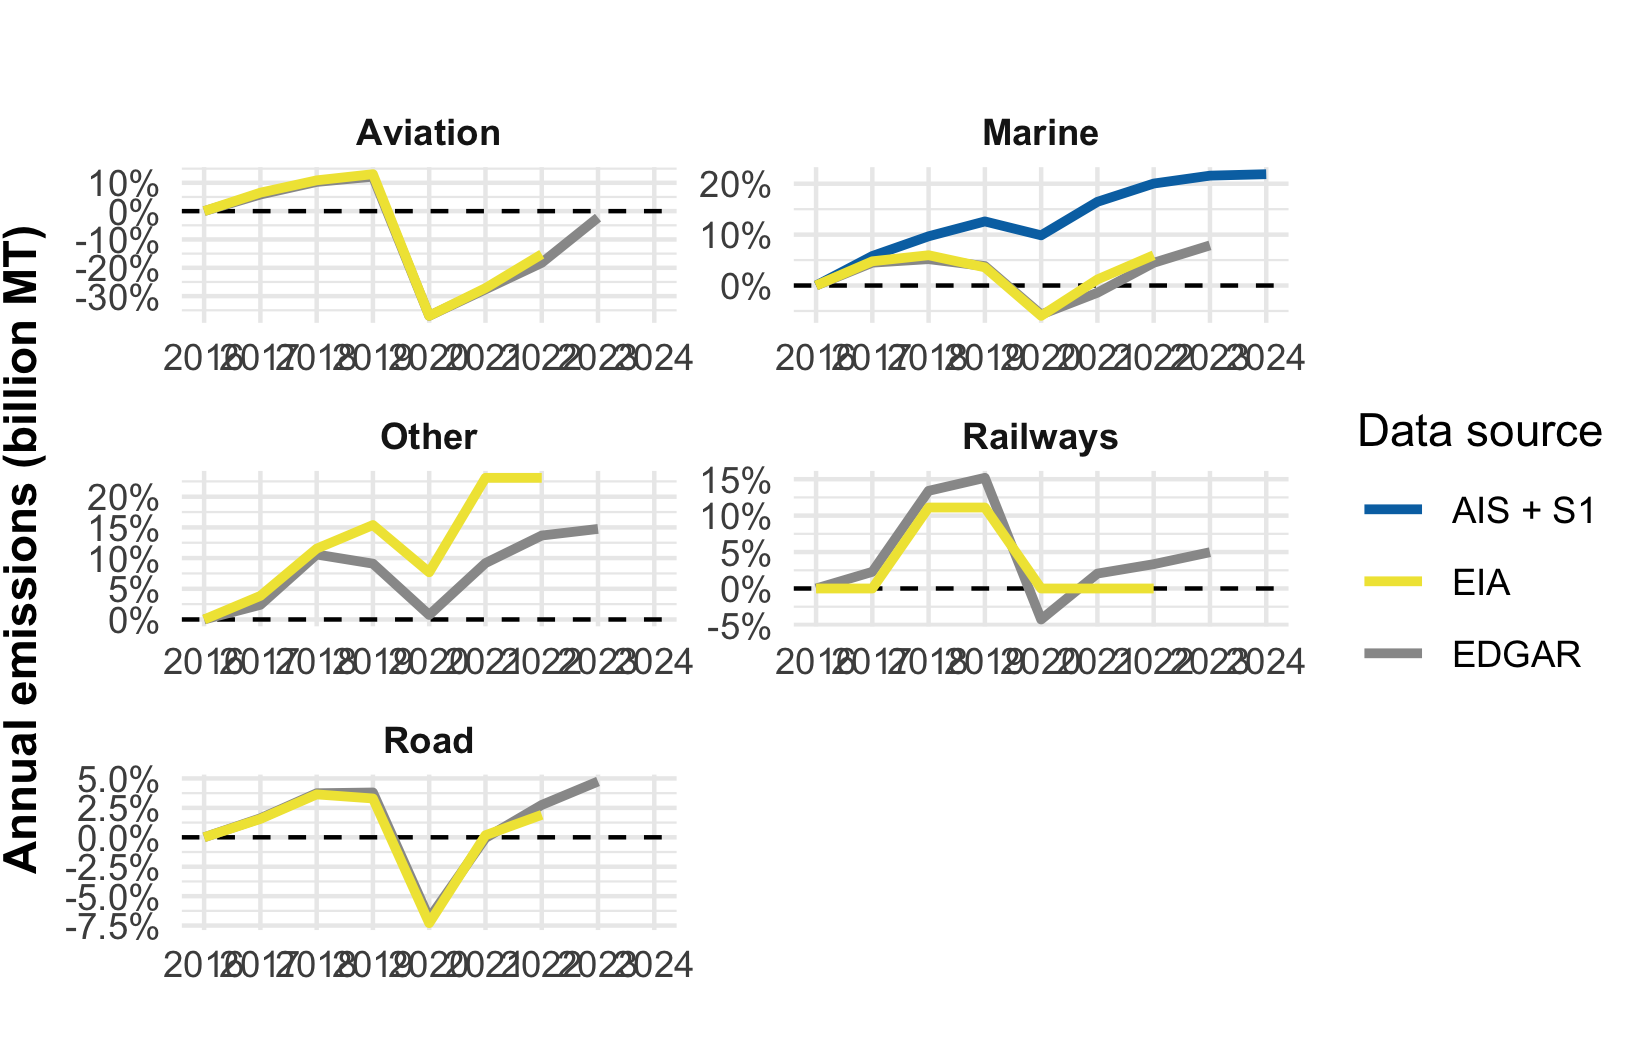
\includegraphics{figures/unnamed-chunk-11-1.png}

\begin{longtable}[]{@{}
  >{\raggedright\arraybackslash}p{(\columnwidth - 8\tabcolsep) * \real{0.3235}}
  >{\raggedleft\arraybackslash}p{(\columnwidth - 8\tabcolsep) * \real{0.0882}}
  >{\raggedleft\arraybackslash}p{(\columnwidth - 8\tabcolsep) * \real{0.0882}}
  >{\raggedright\arraybackslash}p{(\columnwidth - 8\tabcolsep) * \real{0.2794}}
  >{\raggedright\arraybackslash}p{(\columnwidth - 8\tabcolsep) * \real{0.2206}}@{}}

\caption{\label{tbl-total-annual-emissions-by-fleet}Total global annual
CO2 emissions (billion metric tonnes) by fleet for 2016 and 2024. The
percent of total 2024 emissions for each fleet is also shown, along with
the percent change from 2016 to 2024 for each fleet.}

\tabularnewline

\toprule\noalign{}
\begin{minipage}[b]{\linewidth}\raggedright
fleet
\end{minipage} & \begin{minipage}[b]{\linewidth}\raggedleft
2016
\end{minipage} & \begin{minipage}[b]{\linewidth}\raggedleft
2024
\end{minipage} & \begin{minipage}[b]{\linewidth}\raggedright
percent\_total\_2024
\end{minipage} & \begin{minipage}[b]{\linewidth}\raggedright
percent\_change
\end{minipage} \\
\midrule\noalign{}
\endhead
\bottomrule\noalign{}
\endlastfoot
AIS (broadcasting) & 0.839 & 1.120 & 85\% & +34\% \\
S1 (non-broadcasting) & 0.245 & 0.199 & 15\% & -19\% \\
AIS + S1 & 1.080 & 1.320 & 100\% & +22\% \\

\end{longtable}

\subsection{Figure 2}\label{figure-2-1}

\begin{figure}[H]

\centering{


\includegraphics{figures/fig-pollutant-maps-1.png}

}

\caption{\label{fig-pollutant-maps}Spatial map of 2024 emissions for
each pollutant, aggregated across the AIS-broadcasting fleet and
non-broadcasting, and shown at a 1x1 degree spatial resolution}

\end{figure}%

\begin{figure}[H]

\centering{


\includegraphics{figures/fig-co2-emissions-time-series-1.png}

}

\caption{\label{fig-co2-emissions-time-series}Time series of monthly
global CO2 emissions, aggregated across AIS-broadcasting vessels and
non-broadcasting vessels.}

\end{figure}%

\begin{figure}[H]

\centering{


\includegraphics{figures/fig-pollutant-time-series-1.png}

}

\caption{\label{fig-pollutant-time-series}Time series of monthly global
emissions for each pollutant, aggregated across AIS-broadcasting vessels
and non-broadcasting vessels.}

\end{figure}%

\begin{figure}[H]

\centering{


\includegraphics{figures/fig-co2-emissions-by-vessel-type-1.png}

}

\caption{\label{fig-co2-emissions-by-vessel-type}Total 2024 CO2
emissions by vessel type for AIS-broadcasting vessels (millions metric
tonnes).}

\end{figure}%

\subsection{Figure 3}\label{figure-3}

\begin{longtable}[]{@{}lr@{}}

\caption{\label{tbl-decomposition-model-performance}Performance metrics
for random forest model that predicts annual CO2 emissions, by vessel
size class and type, using hours and average speed.}

\tabularnewline

\toprule\noalign{}
.metric & .estimate \\
\midrule\noalign{}
\endhead
\bottomrule\noalign{}
\endlastfoot
rsq & 0.998 \\
mape & 63.342 \\
rsq\_trad & 0.998 \\

\end{longtable}

\subsection{Figure 3 panel A}\label{figure-3-panel-a}

\subsection{Figure 3 Panel B}\label{figure-3-panel-b}

\subsection{Figure 3 combined}\label{figure-3-combined}

\begin{figure}[H]

\centering{


\includegraphics{figures/fig-hours-speed-decomposition-1.png}

}

\caption{\label{fig-hours-speed-decomposition}(A) Estimated
decomposition of change in total CO2 emissions from 2016 baseline
(aggregating across both broadcasting and non-broadcasting vessels),
using the random forest model outputs of four different scenarios that
decompose the relative impact of changes in total kW-hours and changes
in average speed ; (B) Observed total kW-hours for AIS-broadcasting
vessels, number of unique vessels, average hours per vessel, and average
main engine power per vessel; (C) Relative change from a 2016 baseline
for observed total kW-hours for AIS-broadcasting vessels, number of
unique vessels, average hours per vessel, and average main engine power
per vessel.}

\end{figure}%

Looking at the observed AIS data, the number of unique vessels increased
by 57\% from 2016 to 2024, while the average number of hours per vessel
increased by only 13\% and the average main engine power per vessel
actually decreased by 17\%. This suggests that most of the observed 39\%
increase in kW-hours from 2016 to 2024 was driven by the increase in
vessels, not by changes in how much each vessel operates or the engine
size of each vessel.

\section{Abstract text with stats}\label{abstract-text-with-stats}

We develop a method for quantifying high-resolution spatiotemporal
marine vessel emissions at a global scale by fusing two unique
satellite-based data sources: 1) Automatic Identification System (AIS)
to estimate vessel-level emissions for the over 665,000 boats that
broadcast their positions using AIS; and 2) synthetic aperture radar
(SAR) data from the Sentinel-1 satellite constellation to estimate
emissions for boats that do not use AIS. We find that vessels emitted
approximately 1.3 billion metric tons of CO2 in 2023, accounting for
15\% of global fossil fuel emissions from the transportation sector. We
also find that marine CO2 emissions increased by 22\% between 2016 and
2023, 5.3 times the increase measured from terrestrial transportation
emissions. Data fusion is critical to getting these numbers right: if
only AIS data were used, the currently accepted state-of- the-art for
measuring vessel emissions, global emissions in 2024 would be
\emph{underestimated} by 15\%, and the increasing trend from 2016 to
2024 would be \emph{overestimated} by 54\%.

\section{Introduction text with
stats}\label{introduction-text-with-stats}

In 2023, the transportation sector was responsible for 21\% of all
emissions globally

\subsection{Social Cost of Carbon externality
text}\label{social-cost-of-carbon-externality-text}

In 2021, the total global value of commercial maritime transportation
was \$6.63 trillion USD. Looking at our emissions estimates, we find
that non-fishing vessels emitted 1.2 billion metric tonnes of CO2. Using
a SCC value of \$283 USD/metric tonne of CO2, this translates to a total
SCC in 2021 of \$USD 340 billion USD for emissions from the marine
transportation sector, representing 5\% of the total value of goods
transported by maritime trade.

\section{Supplementary tables}\label{supplementary-tables}

\subsection{Summary of 2016 and 2024 emissions, by pollutant and data
source}\label{summary-of-2016-and-2024-emissions-by-pollutant-and-data-source}

\subsection{Underestimation of 2024 emissions using only AIS data, and
overestimation of 2016 to 2024 emissions trend using only AIS data, by
pollutant.}\label{underestimation-of-2024-emissions-using-only-ais-data-and-overestimation-of-2016-to-2024-emissions-trend-using-only-ais-data-by-pollutant.}

\section{Supplementary figures}\label{supplementary-figures}

\begin{figure}[H]

\centering{

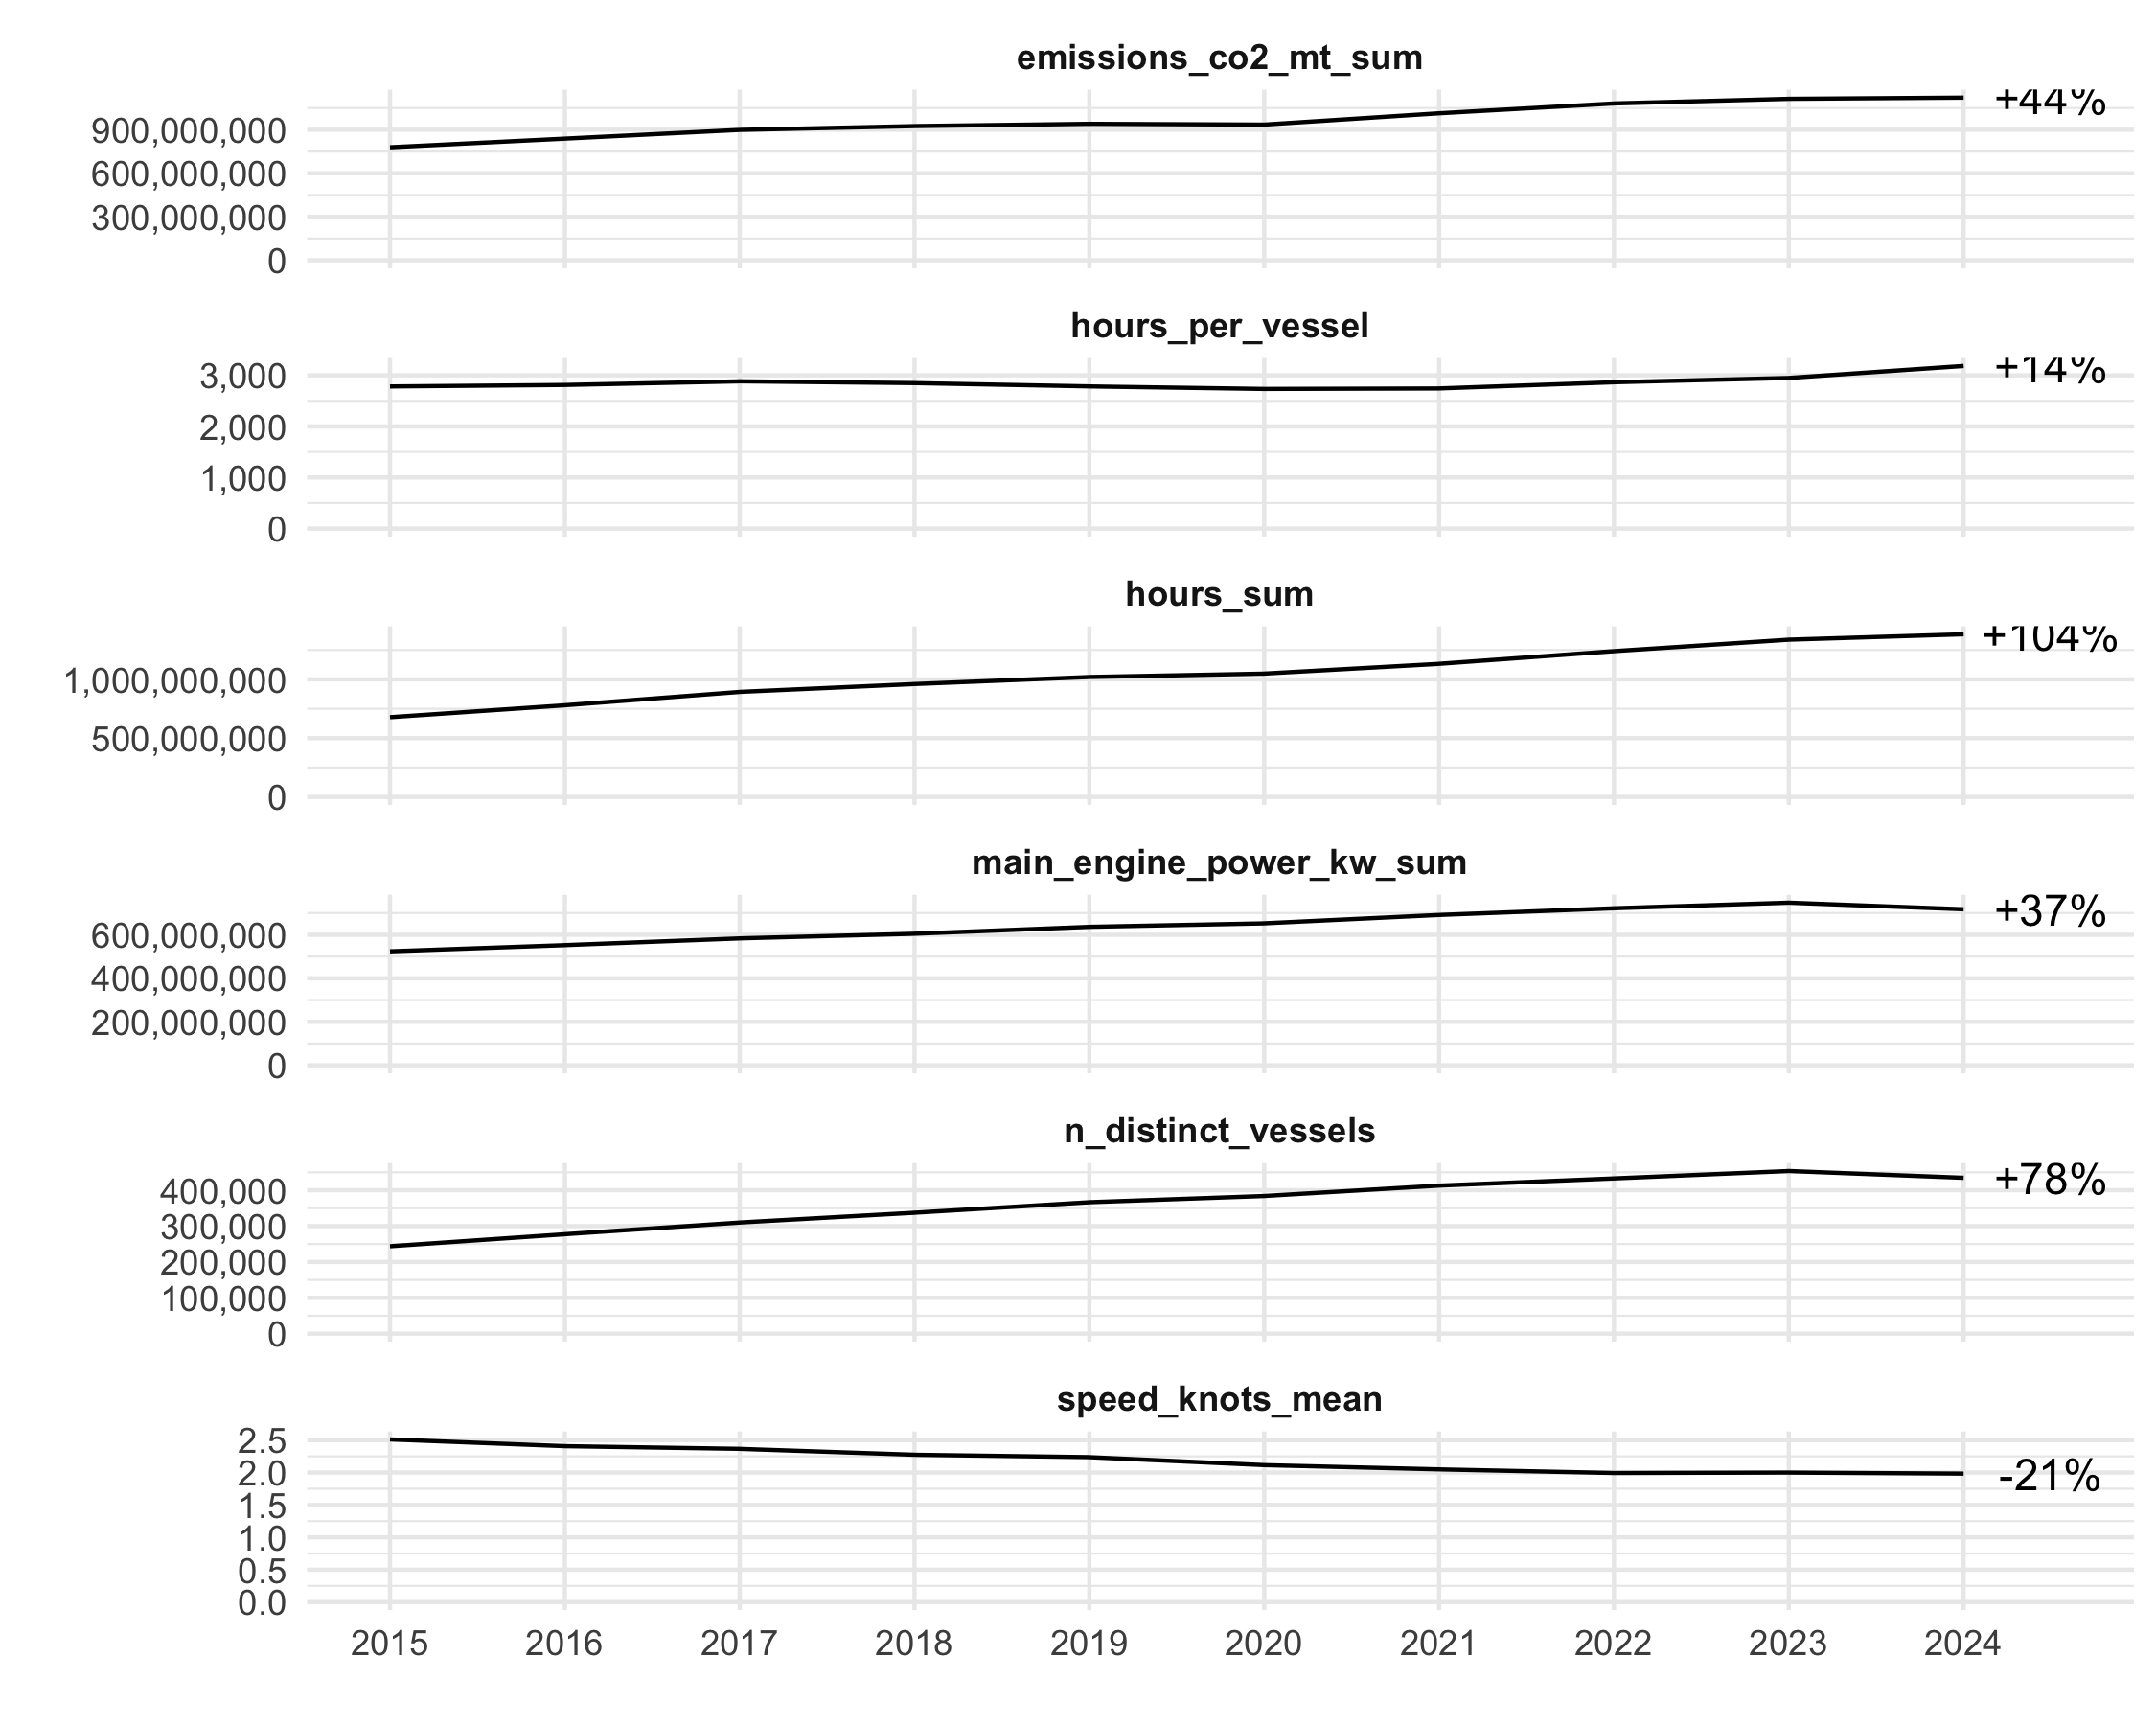
\includegraphics{figures/fig-total-annual-unique-vessels-hours-power-1.png}

}

\caption{\label{fig-total-annual-unique-vessels-hours-power}Annual total
CO2 emissions (metric tonnes); total operating hours; total engine power
across vessels (killowatt); number distinct operating vessels; and
average speed; across all AIS-broadcasting. The percent change from 2015
to 2024 is shown next to each line.}

\end{figure}%

\begin{figure}[H]

\centering{

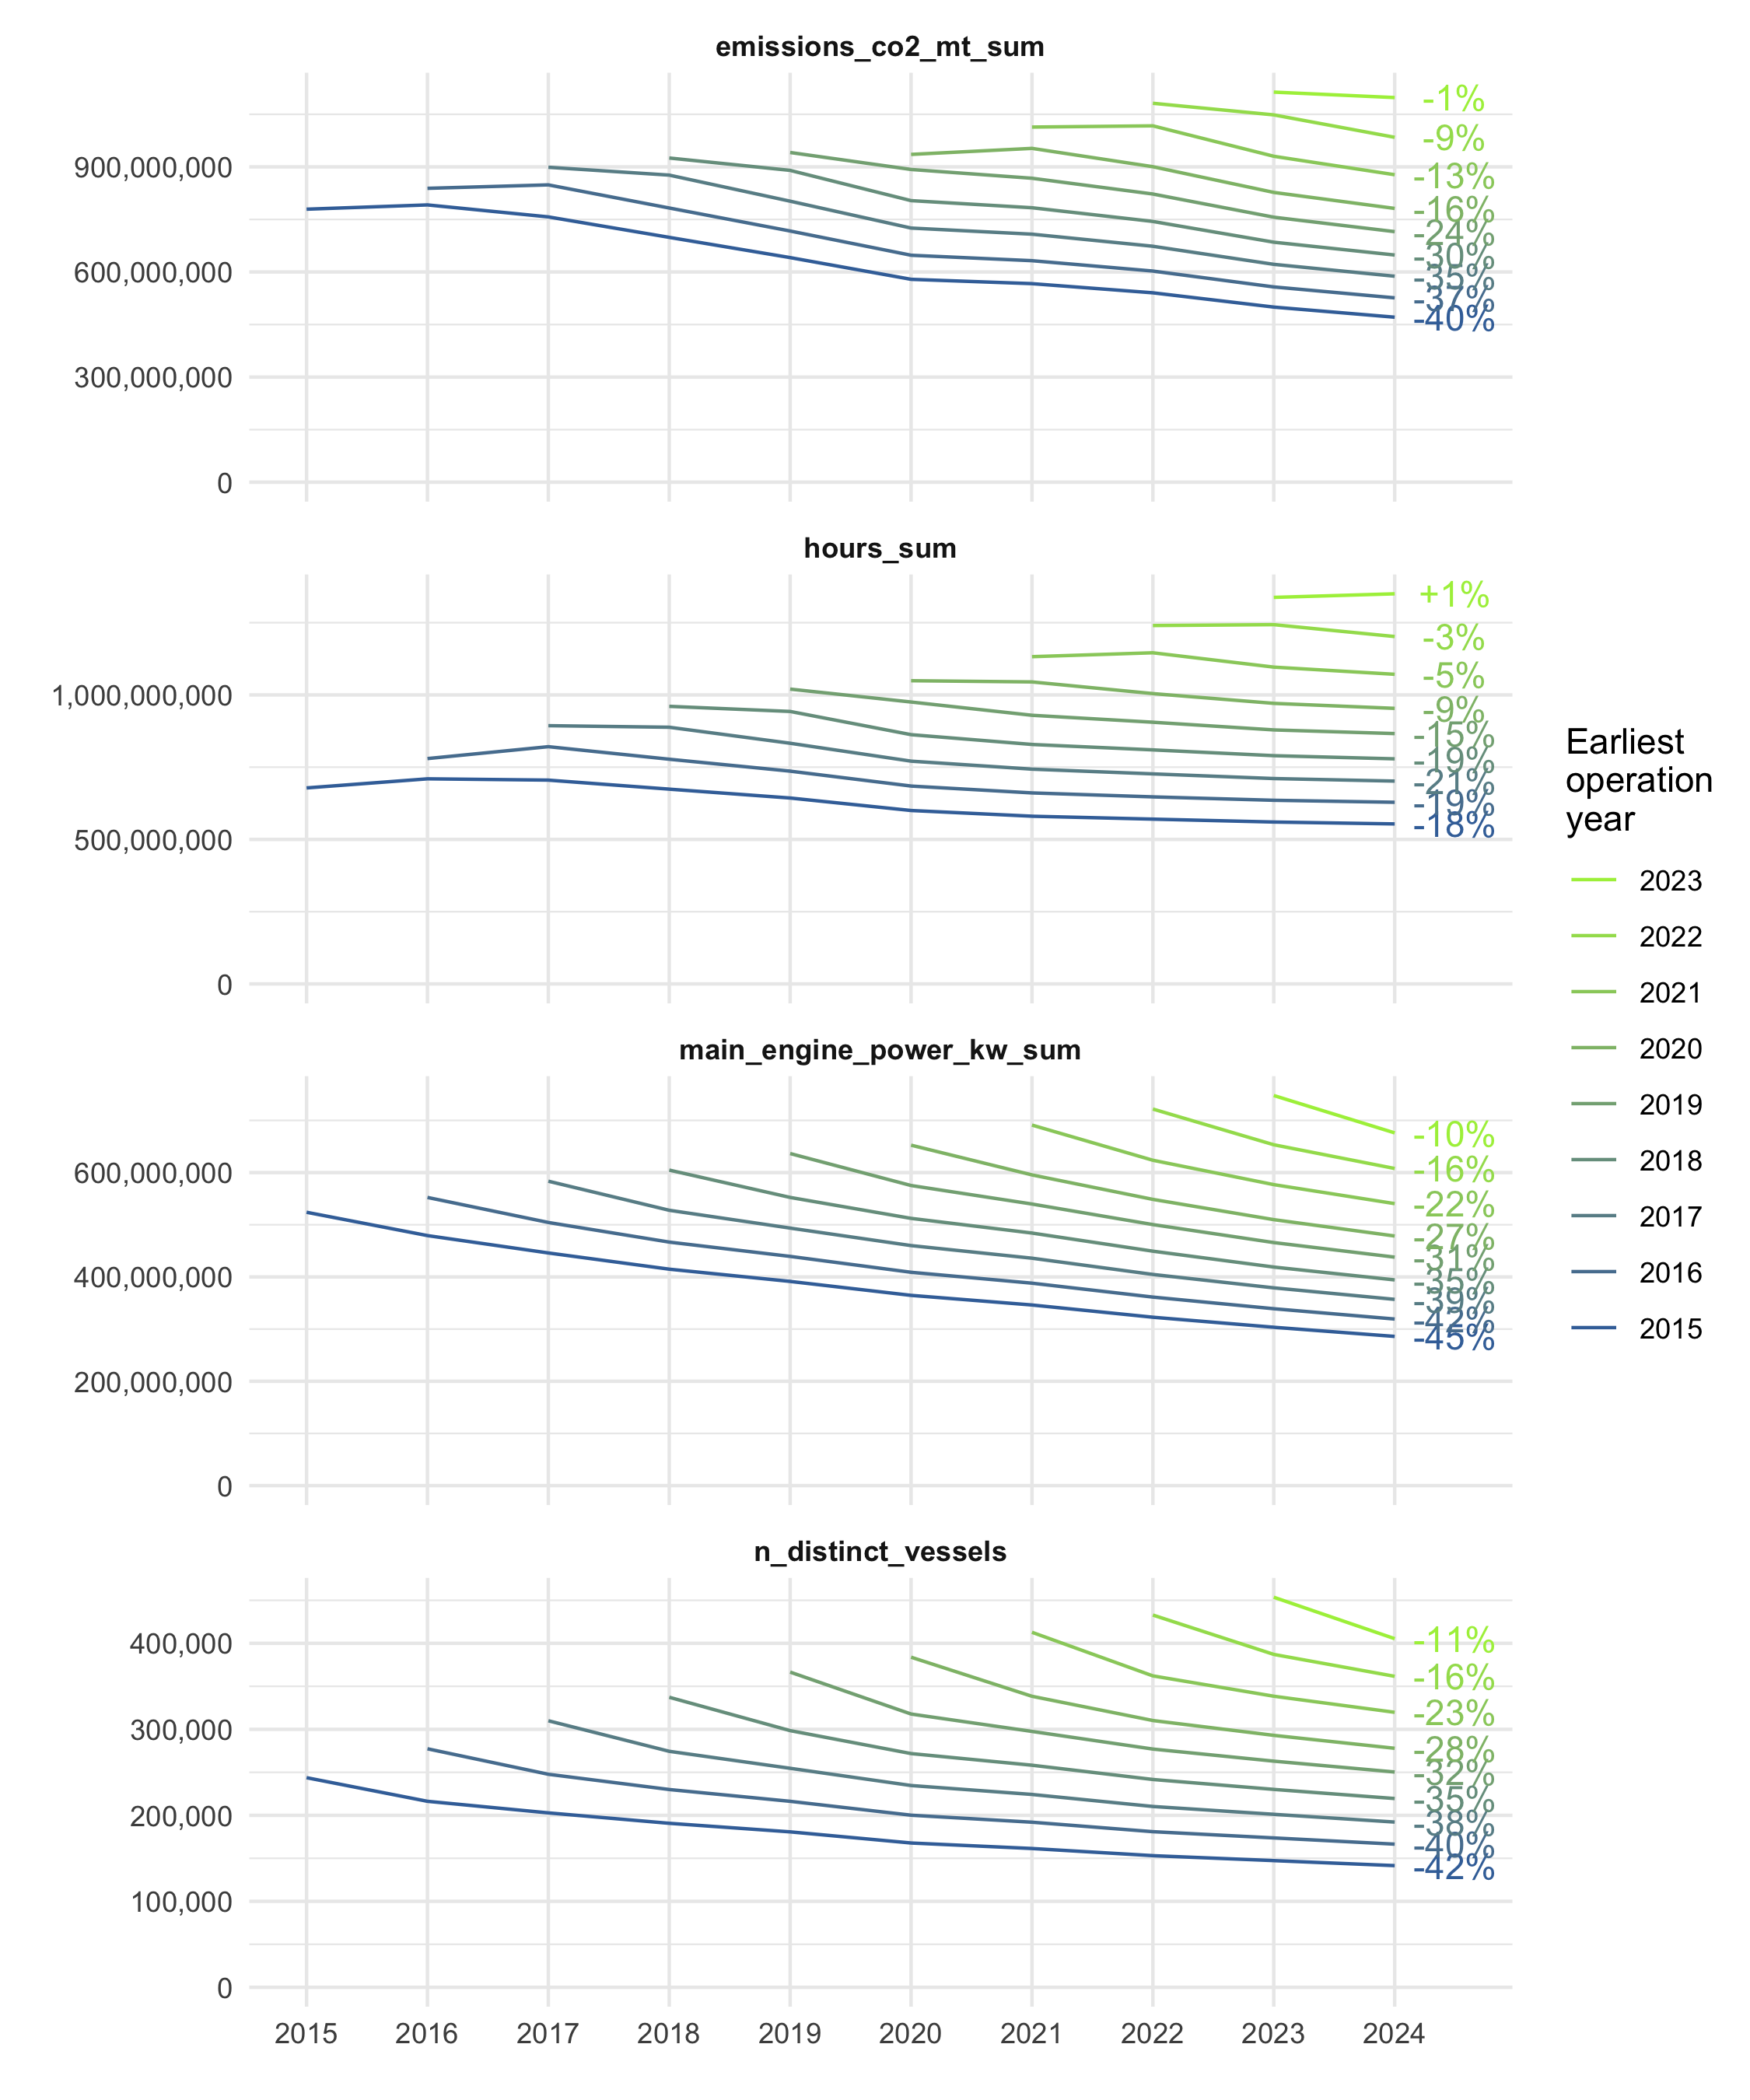
\includegraphics{figures/fig-total-indicators-by-earliest-operation-year-1.png}

}

\caption{\label{fig-total-indicators-by-earliest-operation-year}Total
global CO2 emissions; number unique vessels; operating hours; and total
main engine power for the set of AIS-broadcasting that have been
operating since a given year, where each line is colored by the earliest
operation year. The percent change from the earliest year to 2024 is
shown next to its line.}

\end{figure}%

\begin{figure}[H]

\centering{

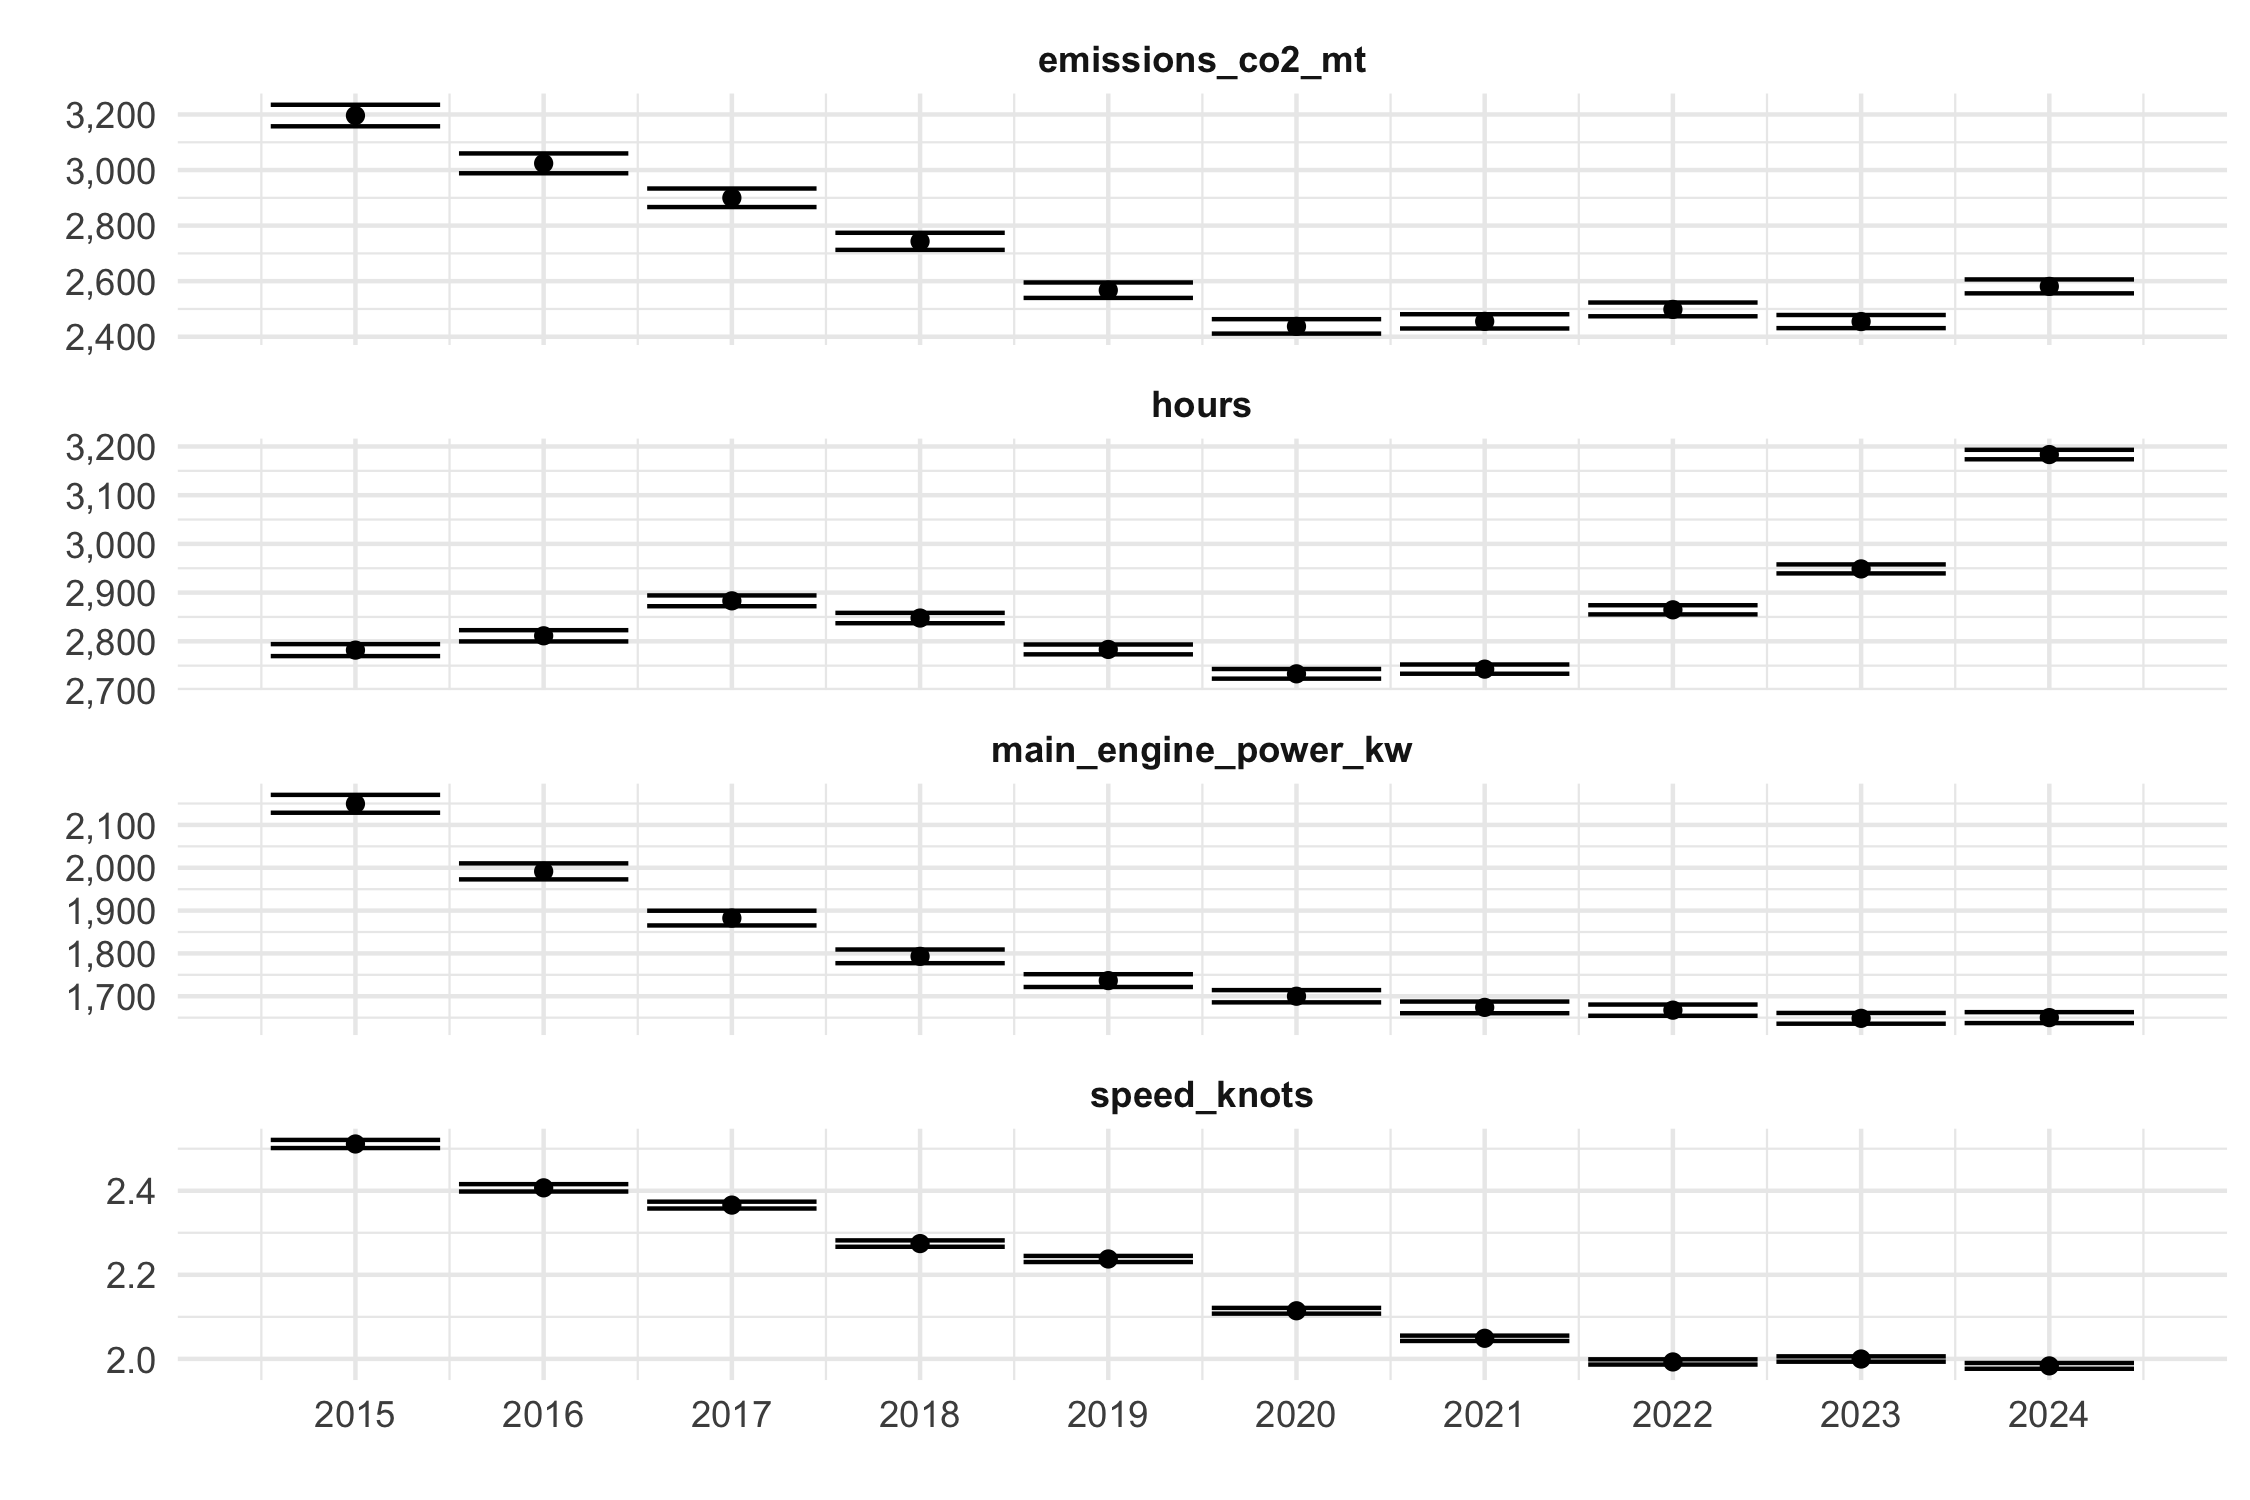
\includegraphics{figures/fig-individual-distribution-annual-emissions-hours-power-1.png}

}

\caption{\label{fig-individual-distribution-annual-emissions-hours-power}Annual
distributions of individual per-vessel CO2 emissions (metric tonnes);
operating hours; main engine power (killowatts); and average speed
(knots). The point shows the mean value, and the error bars show +/- two
standard errors.}

\end{figure}%

\begin{figure}[H]

\centering{

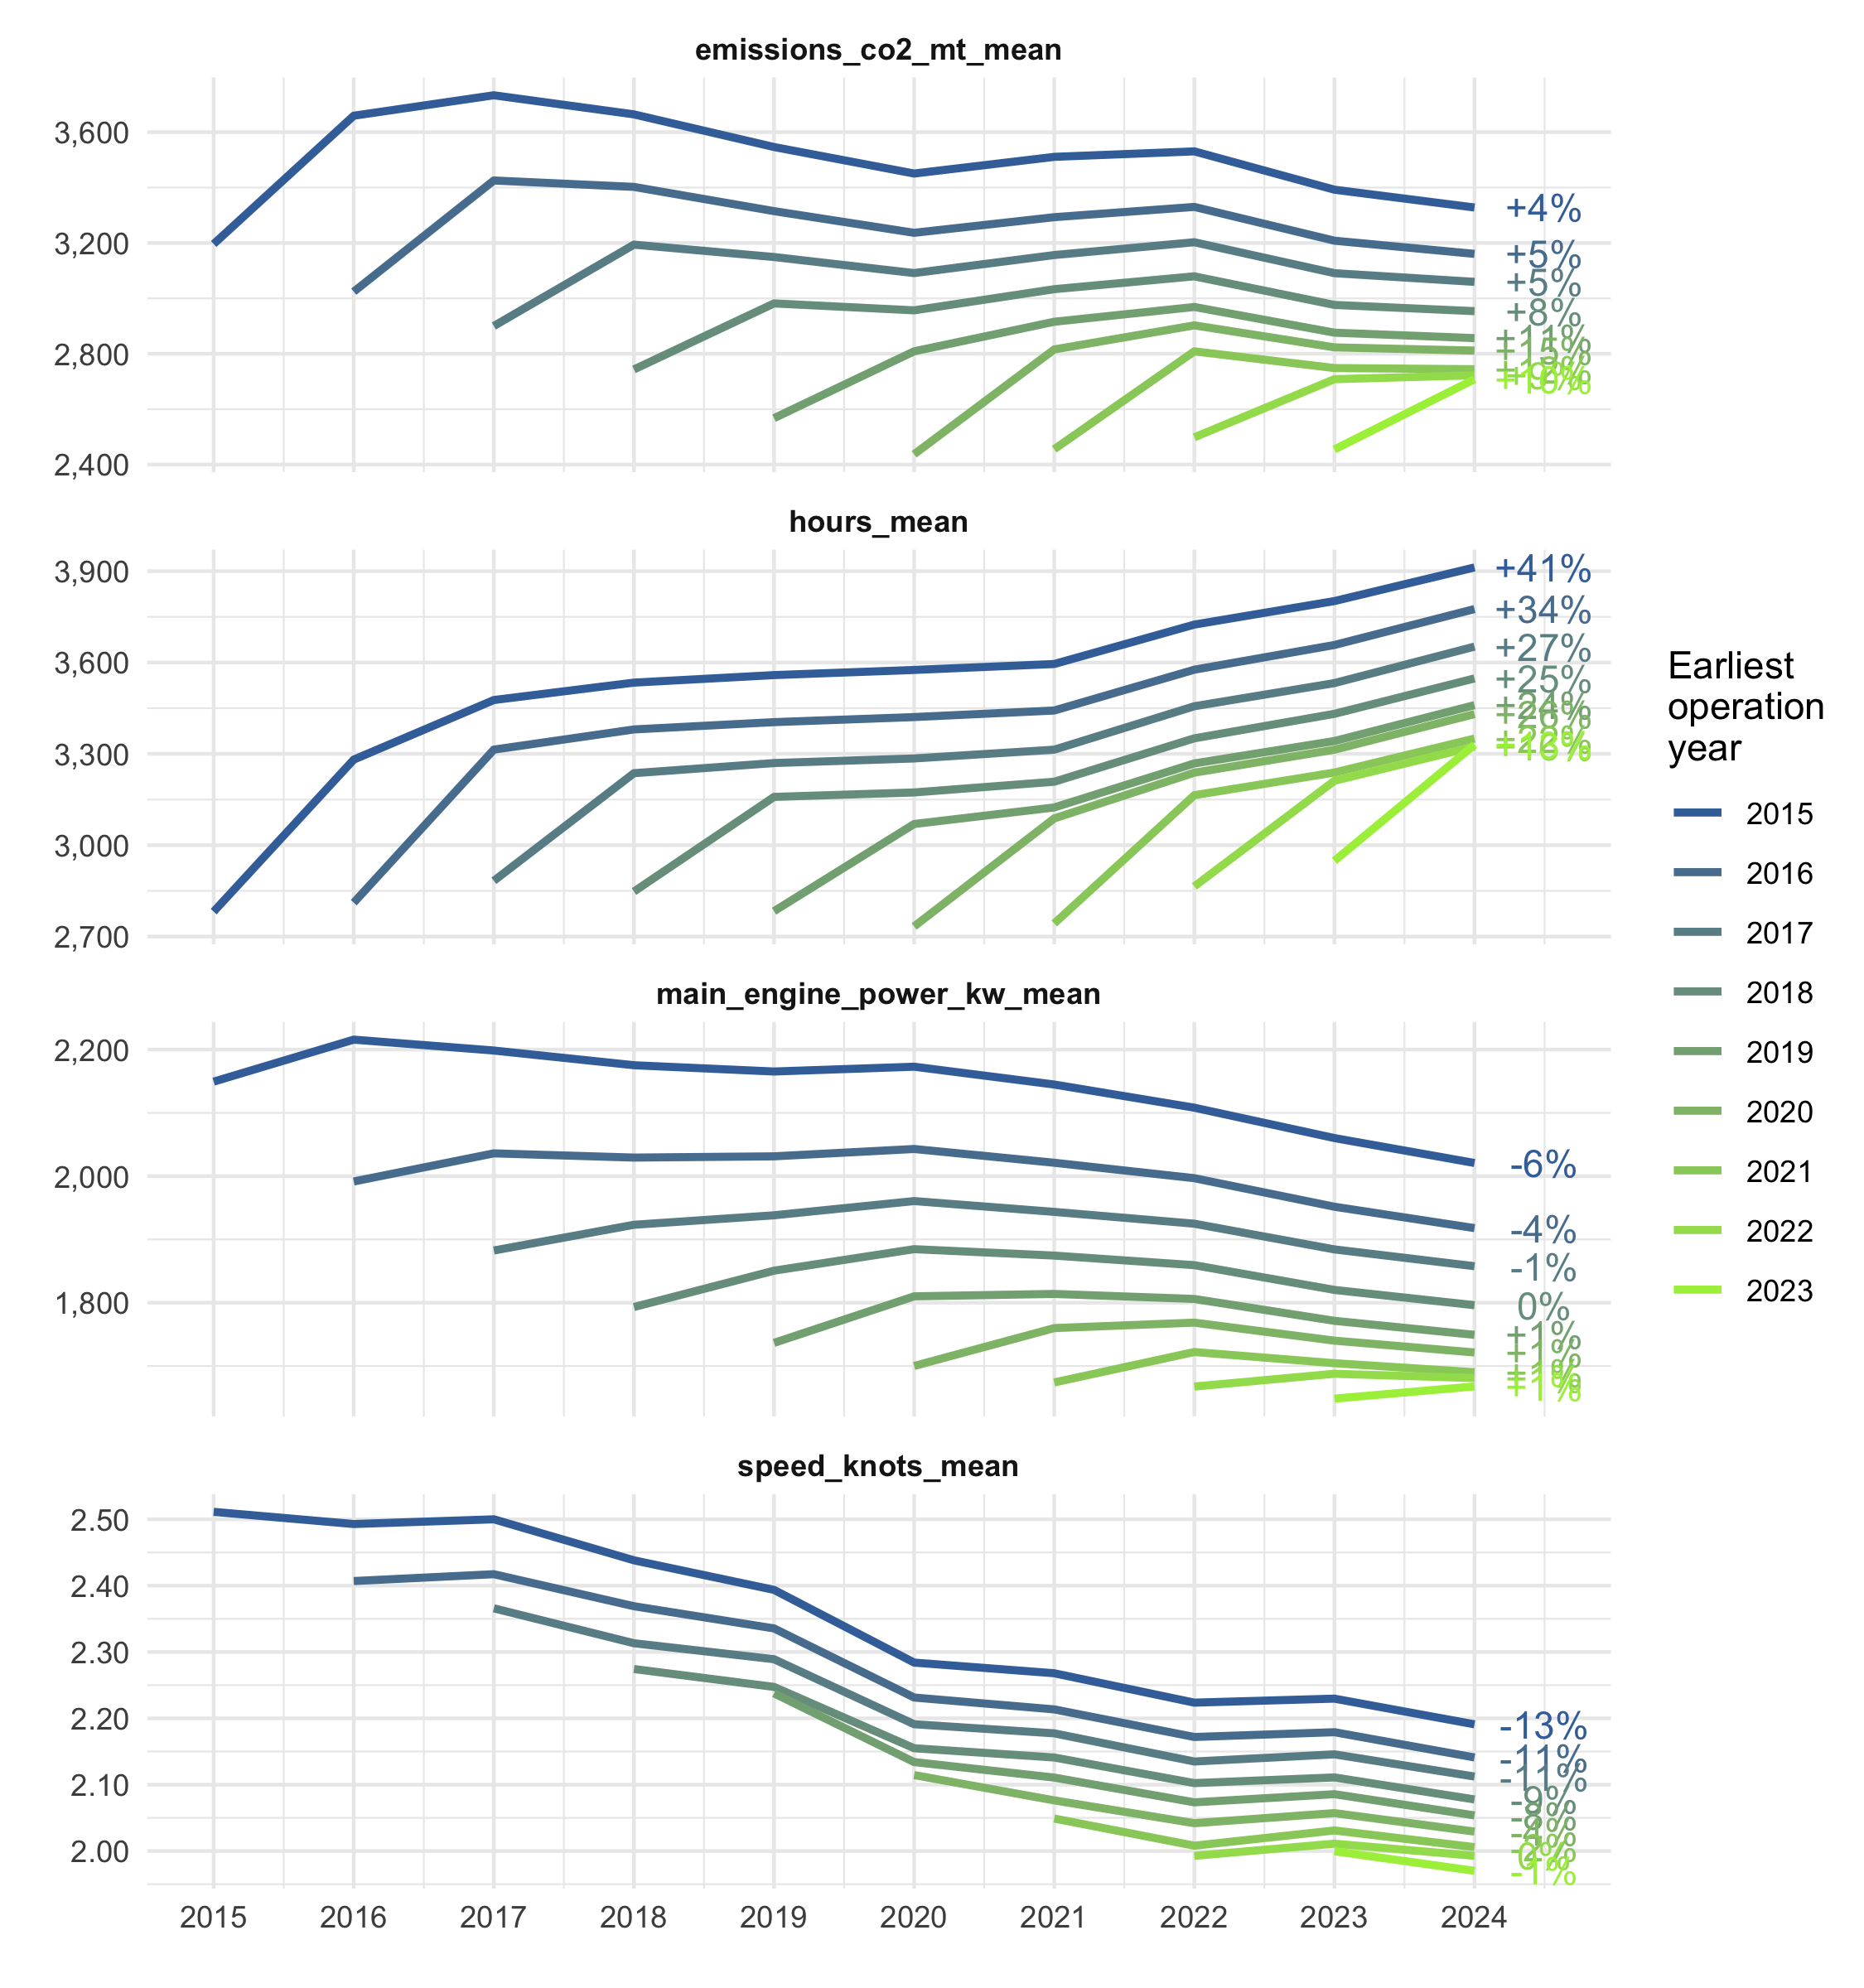
\includegraphics{figures/fig-individual-distribution-annual-emissions-hours-power-by-earliest-operation-year-1.png}

}

\caption{\label{fig-individual-distribution-annual-emissions-hours-power-by-earliest-operation-year}Annual
mean of individual per-vessel CO2 emissions (metric tonnes); operating
hours; main engine power (killowatts); and average speed (knots) for the
set of AIS-broadcasting that have been operating since a given year,
where each line is colored by the earliest operation year. The percent
change from the earliest year to 2024 is shown next to its line.}

\end{figure}%

\begin{figure}[H]

\centering{

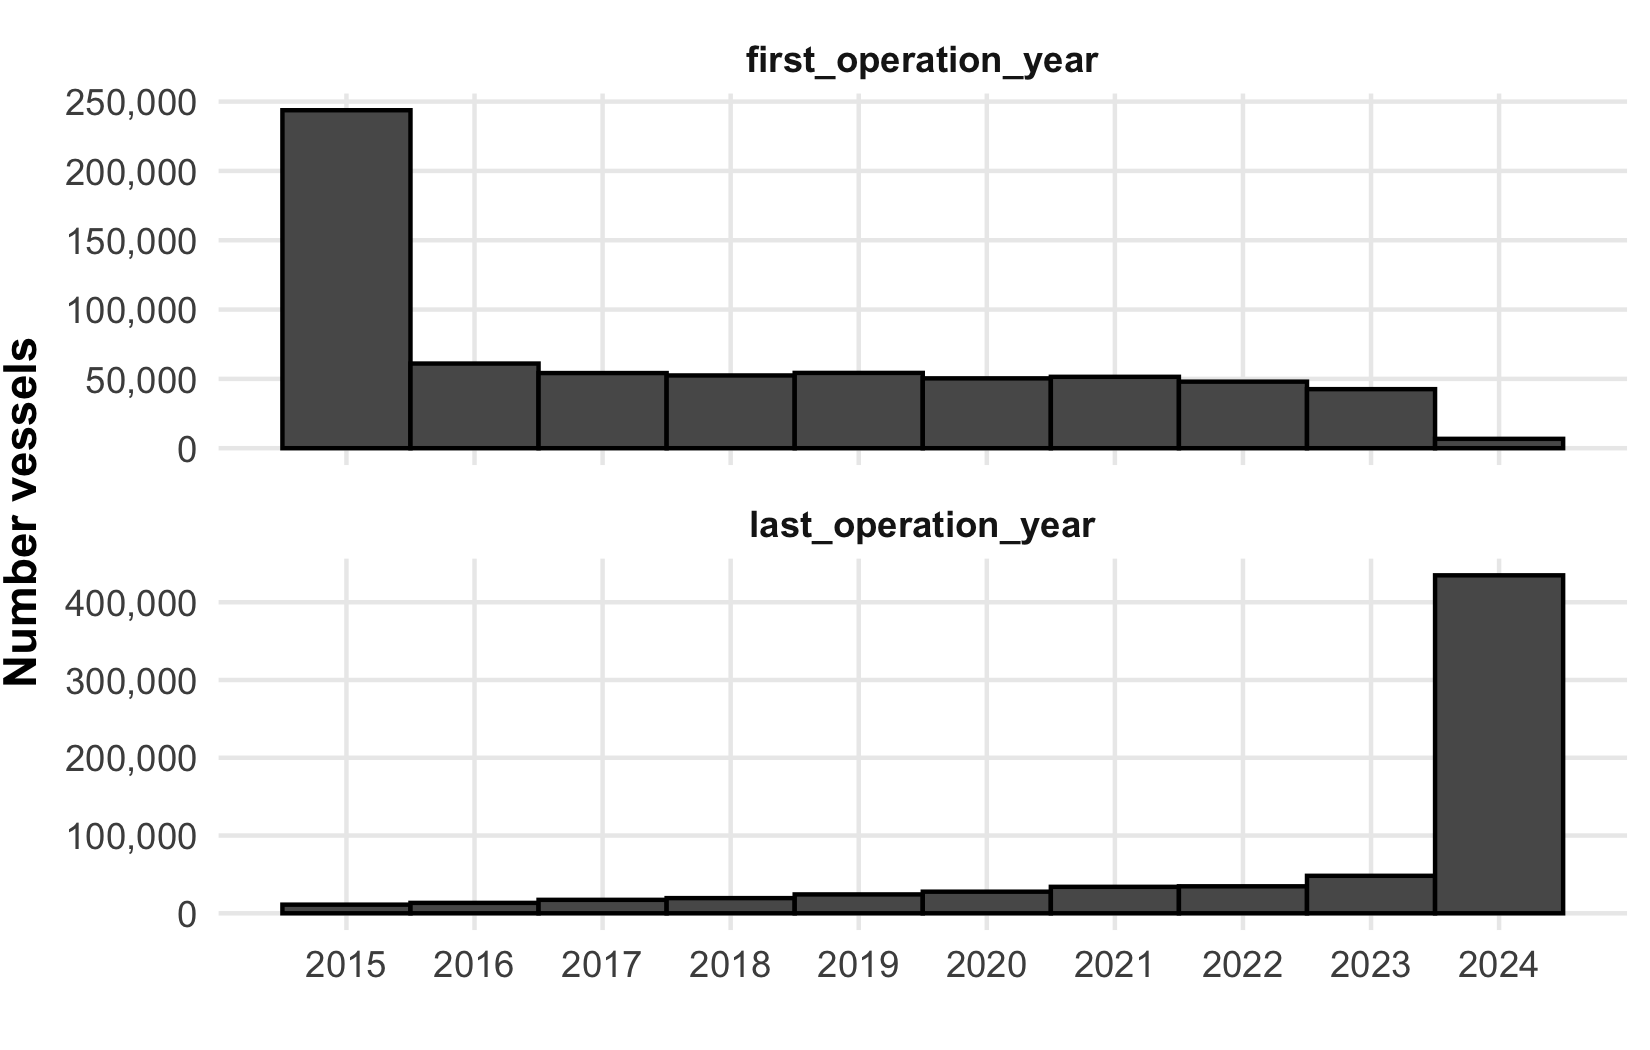
\includegraphics{figures/fig-first-last-operation-year-histogram-1.png}

}

\caption{\label{fig-first-last-operation-year-histogram}Histograms
showing the distribution of the first and last operation year of each
vessel.}

\end{figure}%

\begin{figure}[H]

\centering{

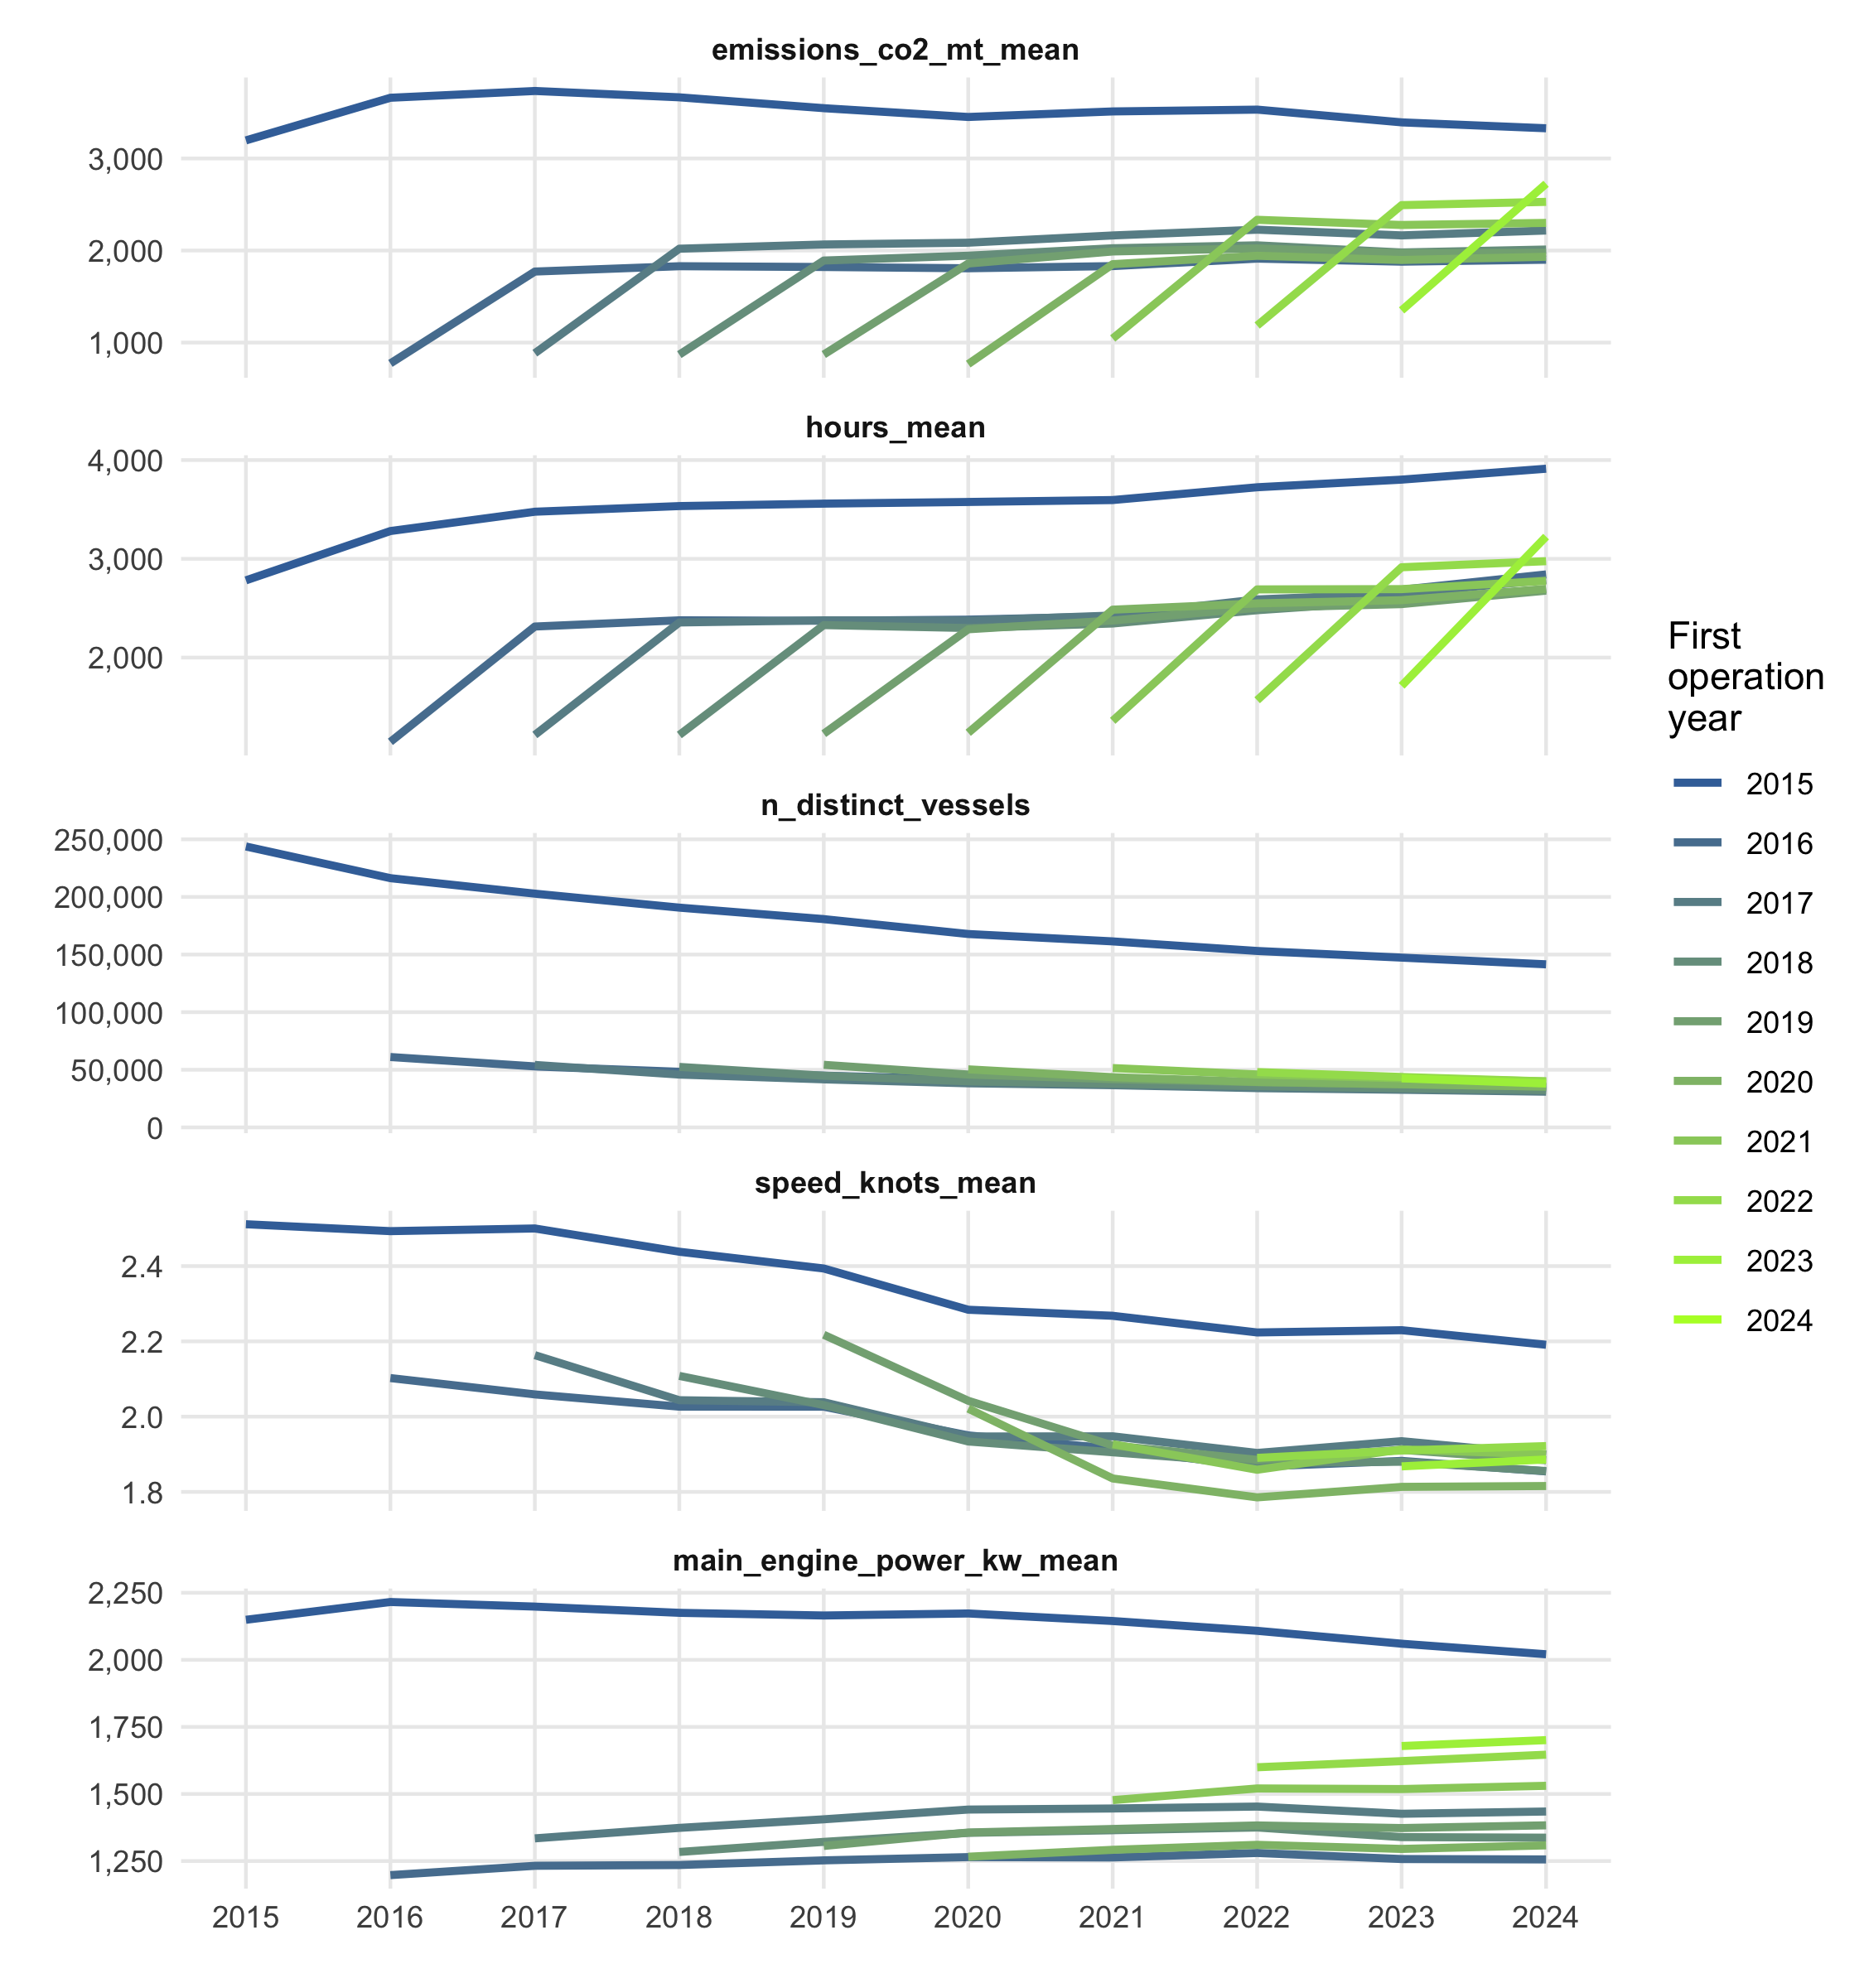
\includegraphics{figures/fig-individual-distribution-annual-emissions-hours-power-by-first-year-1.png}

}

\caption{\label{fig-individual-distribution-annual-emissions-hours-power-by-first-year}Annual
mean of individual per-vessel CO2 emissions (metric tonnes); mean
per-vessel operating hours; mean per-vessel main engine power
(killowatts); mean per-vessel speed (knots); and total number of
distinct vessels for the set of AIS-broadcasting for each first year of
operation, where each line is colored by the first operation year.}

\end{figure}%

\begin{figure}[H]

\centering{

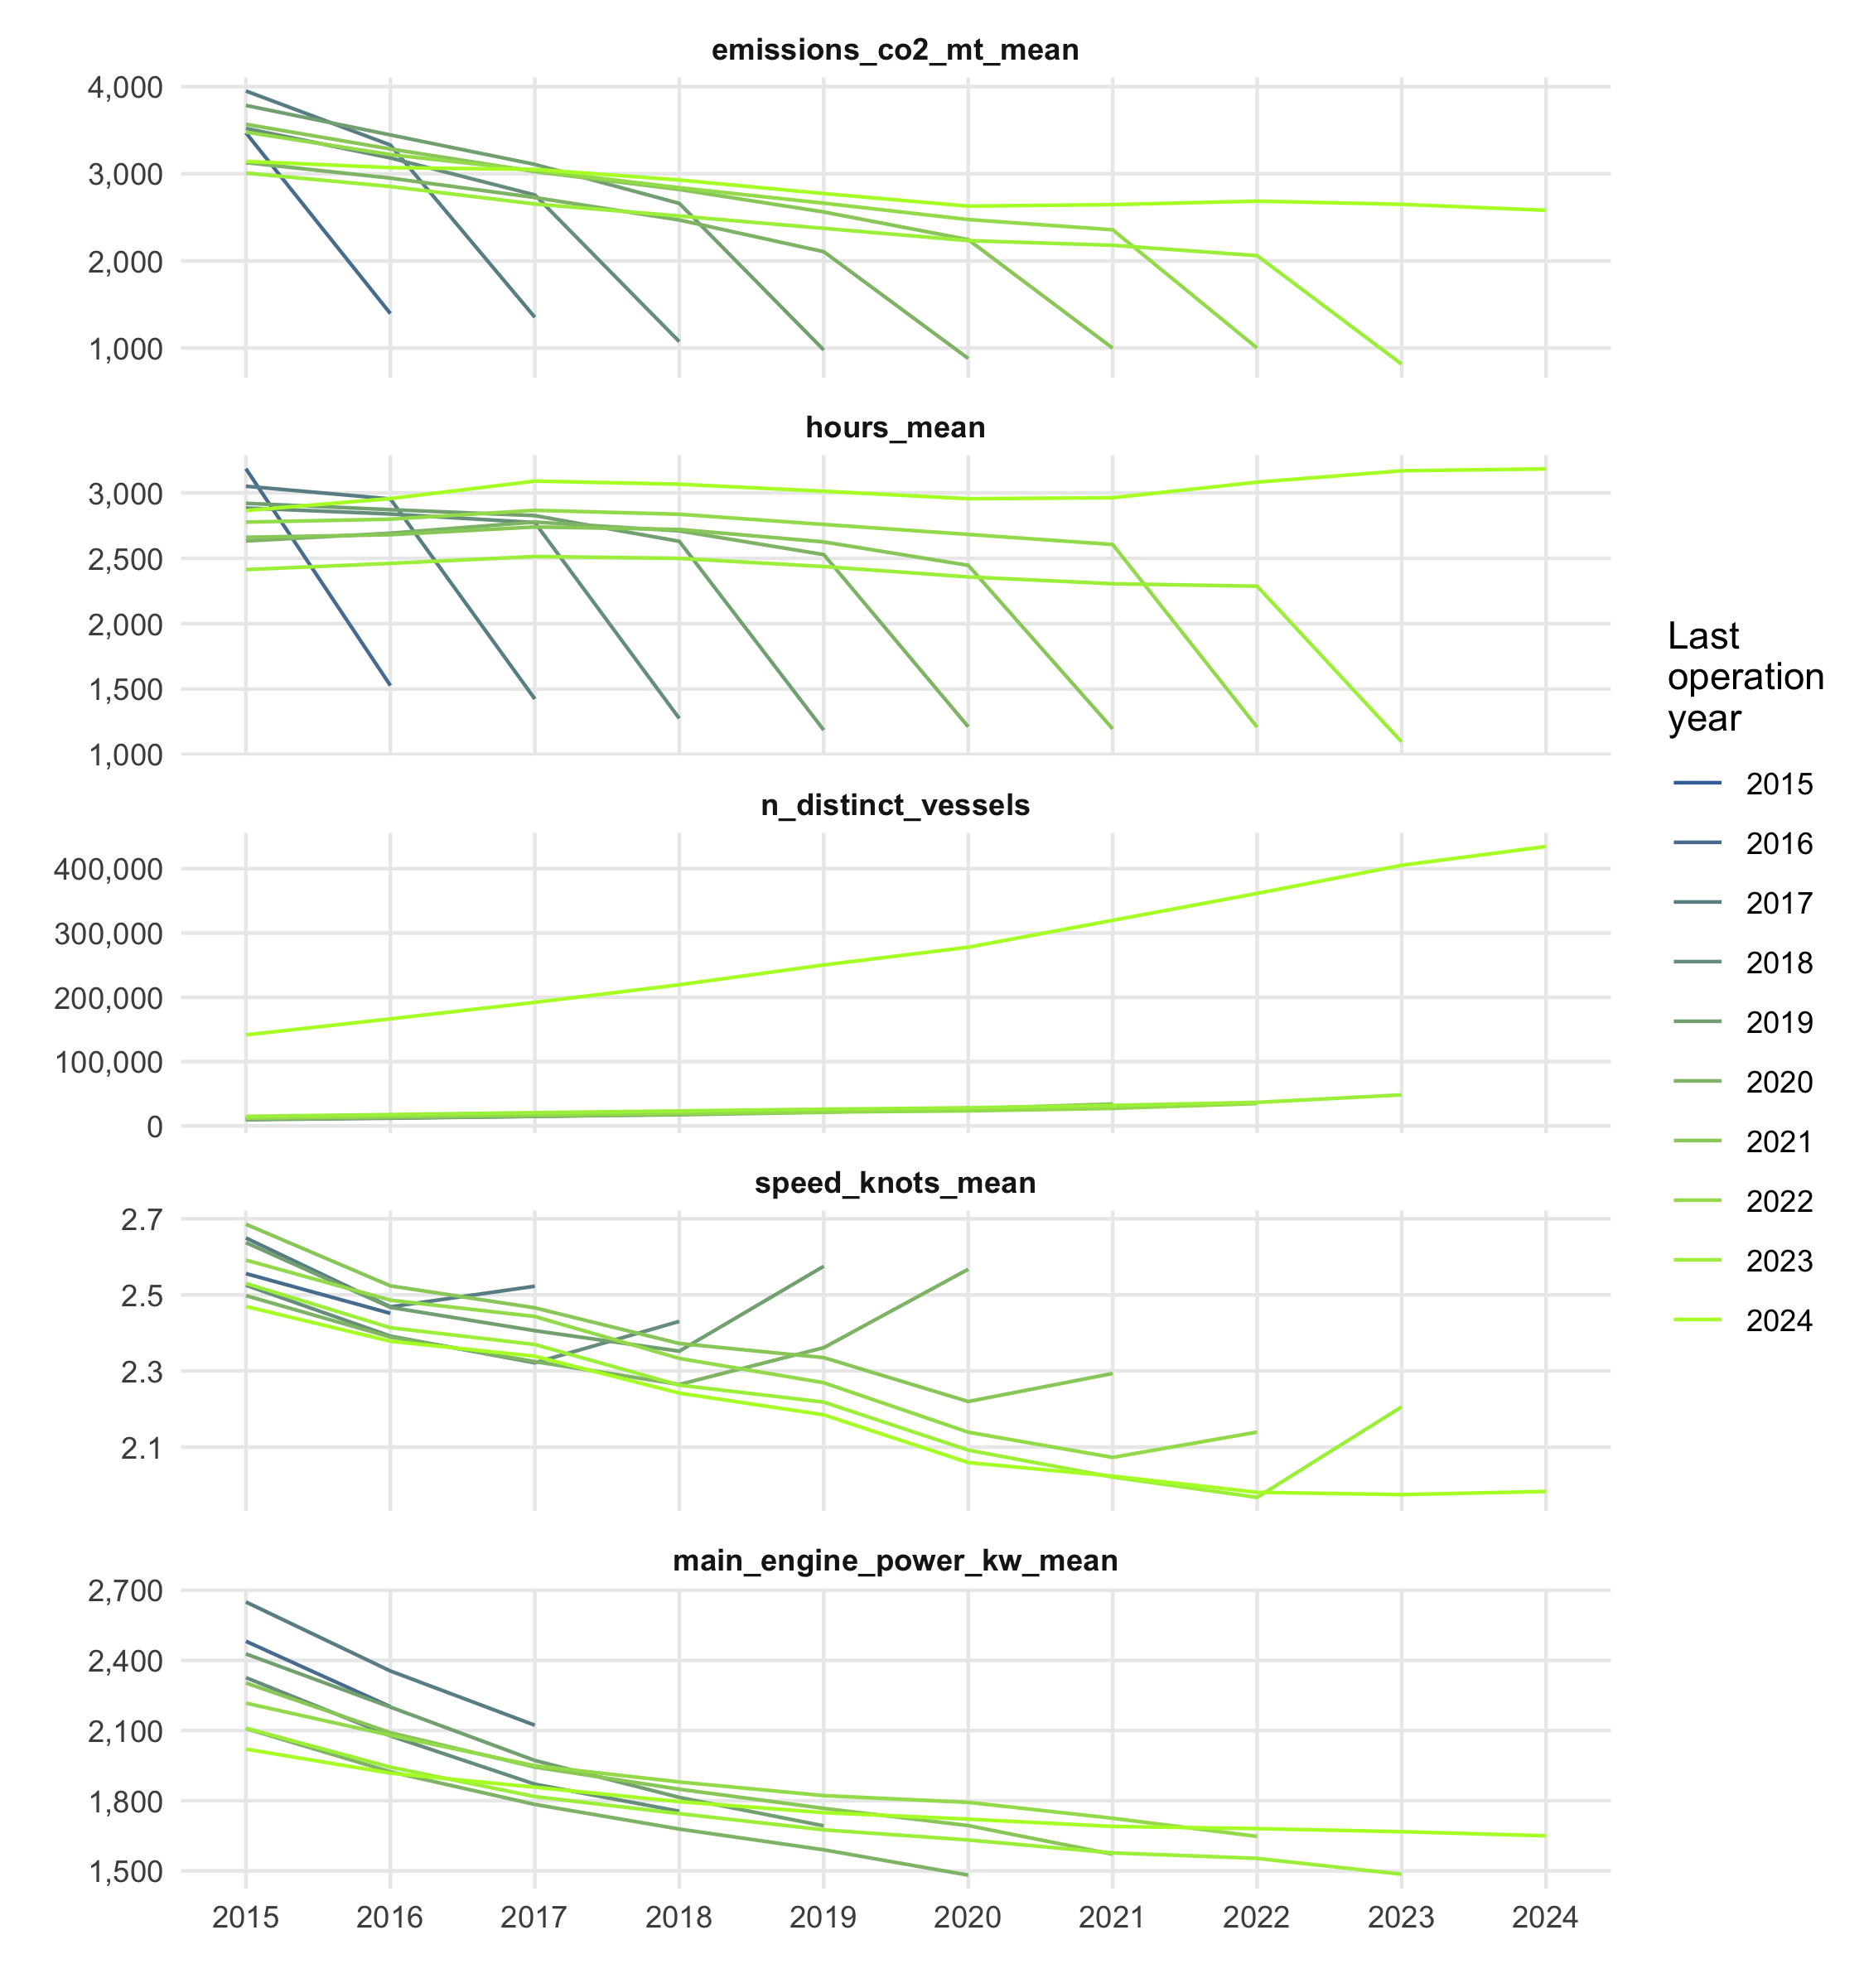
\includegraphics{figures/fig-individual-distribution-annual-emissions-hours-power-by-last-year-1.png}

}

\caption{\label{fig-individual-distribution-annual-emissions-hours-power-by-last-year}Annual
mean of individual per-vessel CO2 emissions (metric tonnes); mean
per-vessel operating hours; mean per-vessel main engine power
(killowatts); mean per-vessel speed (knots); and total number of
distinct vessels for the set of AIS-broadcasting for each last year of
operation, where each line is colored by the last operation year.}

\end{figure}%

\begin{figure}[H]

\centering{


\includegraphics{figures/fig-annual-emissions-by-ais-receiver-type-1.png}

}

\caption{\label{fig-annual-emissions-by-ais-receiver-type}Annual total
CO2 emissions (metric tonnes) by the AIS-broadcasting fleet,
disaggregated by AIS receiver type (satellite, terrestrial, and dynamic)
and total aggregated across receiver types. A dashed vertical line is
shown for 2022, the first year in which dynamic AIS was widely adopted.}

\end{figure}%

\begin{figure}[H]

\centering{


\includegraphics{figures/fig-annual-emissions-by-ais-receiver-type-top-flags-1.png}

}

\caption{\label{fig-annual-emissions-by-ais-receiver-type-top-flags}Annual
total CO2 emissions (metric tonnes) by the AIS-broadcasting fleet,
disaggregated by AIS receiver type (satellite, terrestrial, and dynamic)
and total aggregated across receiver types, for the top 10 flags with
the most emissions in 2024. A dashed vertical line is shown for 2022,
the first year in which dynamic AIS was widely adopted.}

\end{figure}%

\begin{figure}[H]

\centering{

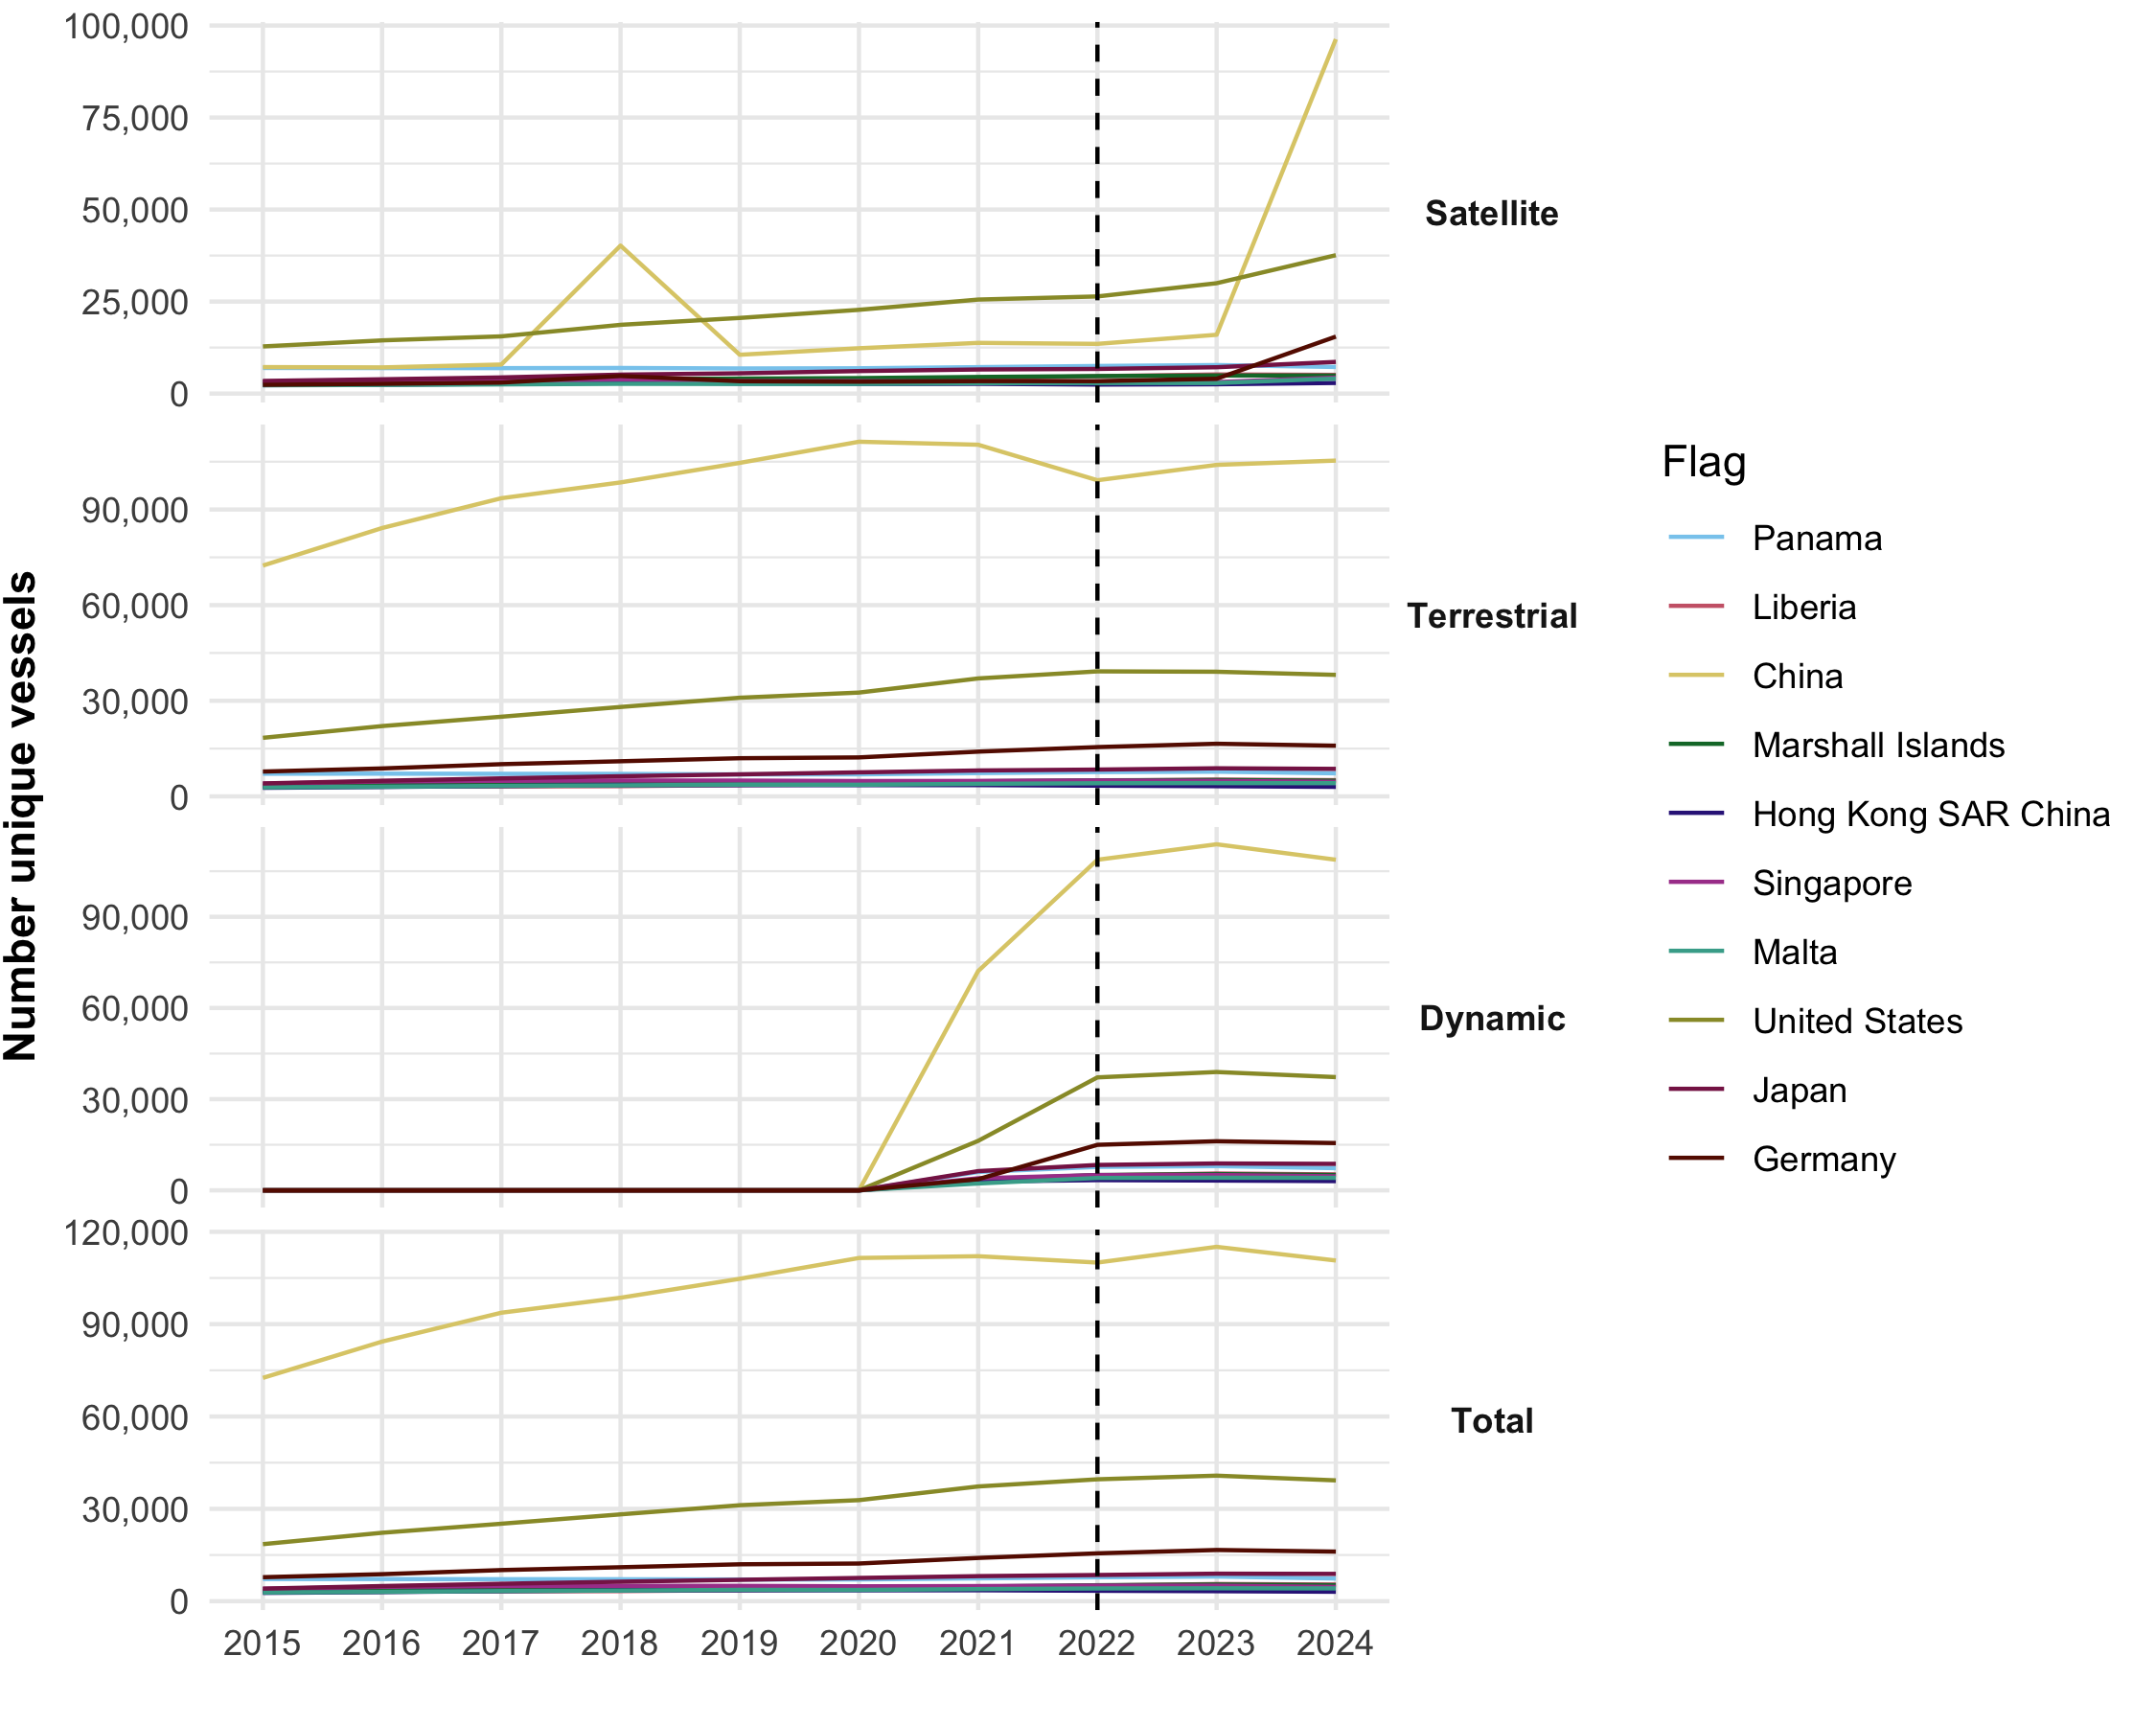
\includegraphics{figures/fig-annual-unique-vessels-by-ais-receiver-type-top-flags-1.png}

}

\caption{\label{fig-annual-unique-vessels-by-ais-receiver-type-top-flags}Annual
unique number of vessels in the AIS-broadcasting fleet, disaggregated by
AIS receiver type (satellite, terrestrial, and dynamic) and total
aggregated across receiver types, for the top 10 flags with the most
emissions in 2024. A dashed vertical line is shown for 2022, the first
year in which dynamic AIS was widely adopted.}

\end{figure}%

\begin{figure}[H]

\centering{


\includegraphics{figures/fig-co2-emissions-change-map-by-receiver-type-1.png}

}

\caption{\label{fig-co2-emissions-change-map-by-receiver-type}Spatial
change in CO2 emissions by the AIS-broadcasting fleet between 2016 and
2024 (metric tonnes) by receiver type (satellite, terrestrial, and
dynamic) and total across receiver types, at a 1x1 degree spatial
resolution.}

\end{figure}%

\subsection{Olivier's plots}\label{oliviers-plots}

Following Olivier's complementary materials shared on Slack, we present
the mean values of four parameters defining yearly information for
AIS-broadcasting operating across all years. The data is derived from
the ping-level dataset, thus including emissions associated with both
port stays and trips.

\begin{figure}[H]

\centering{

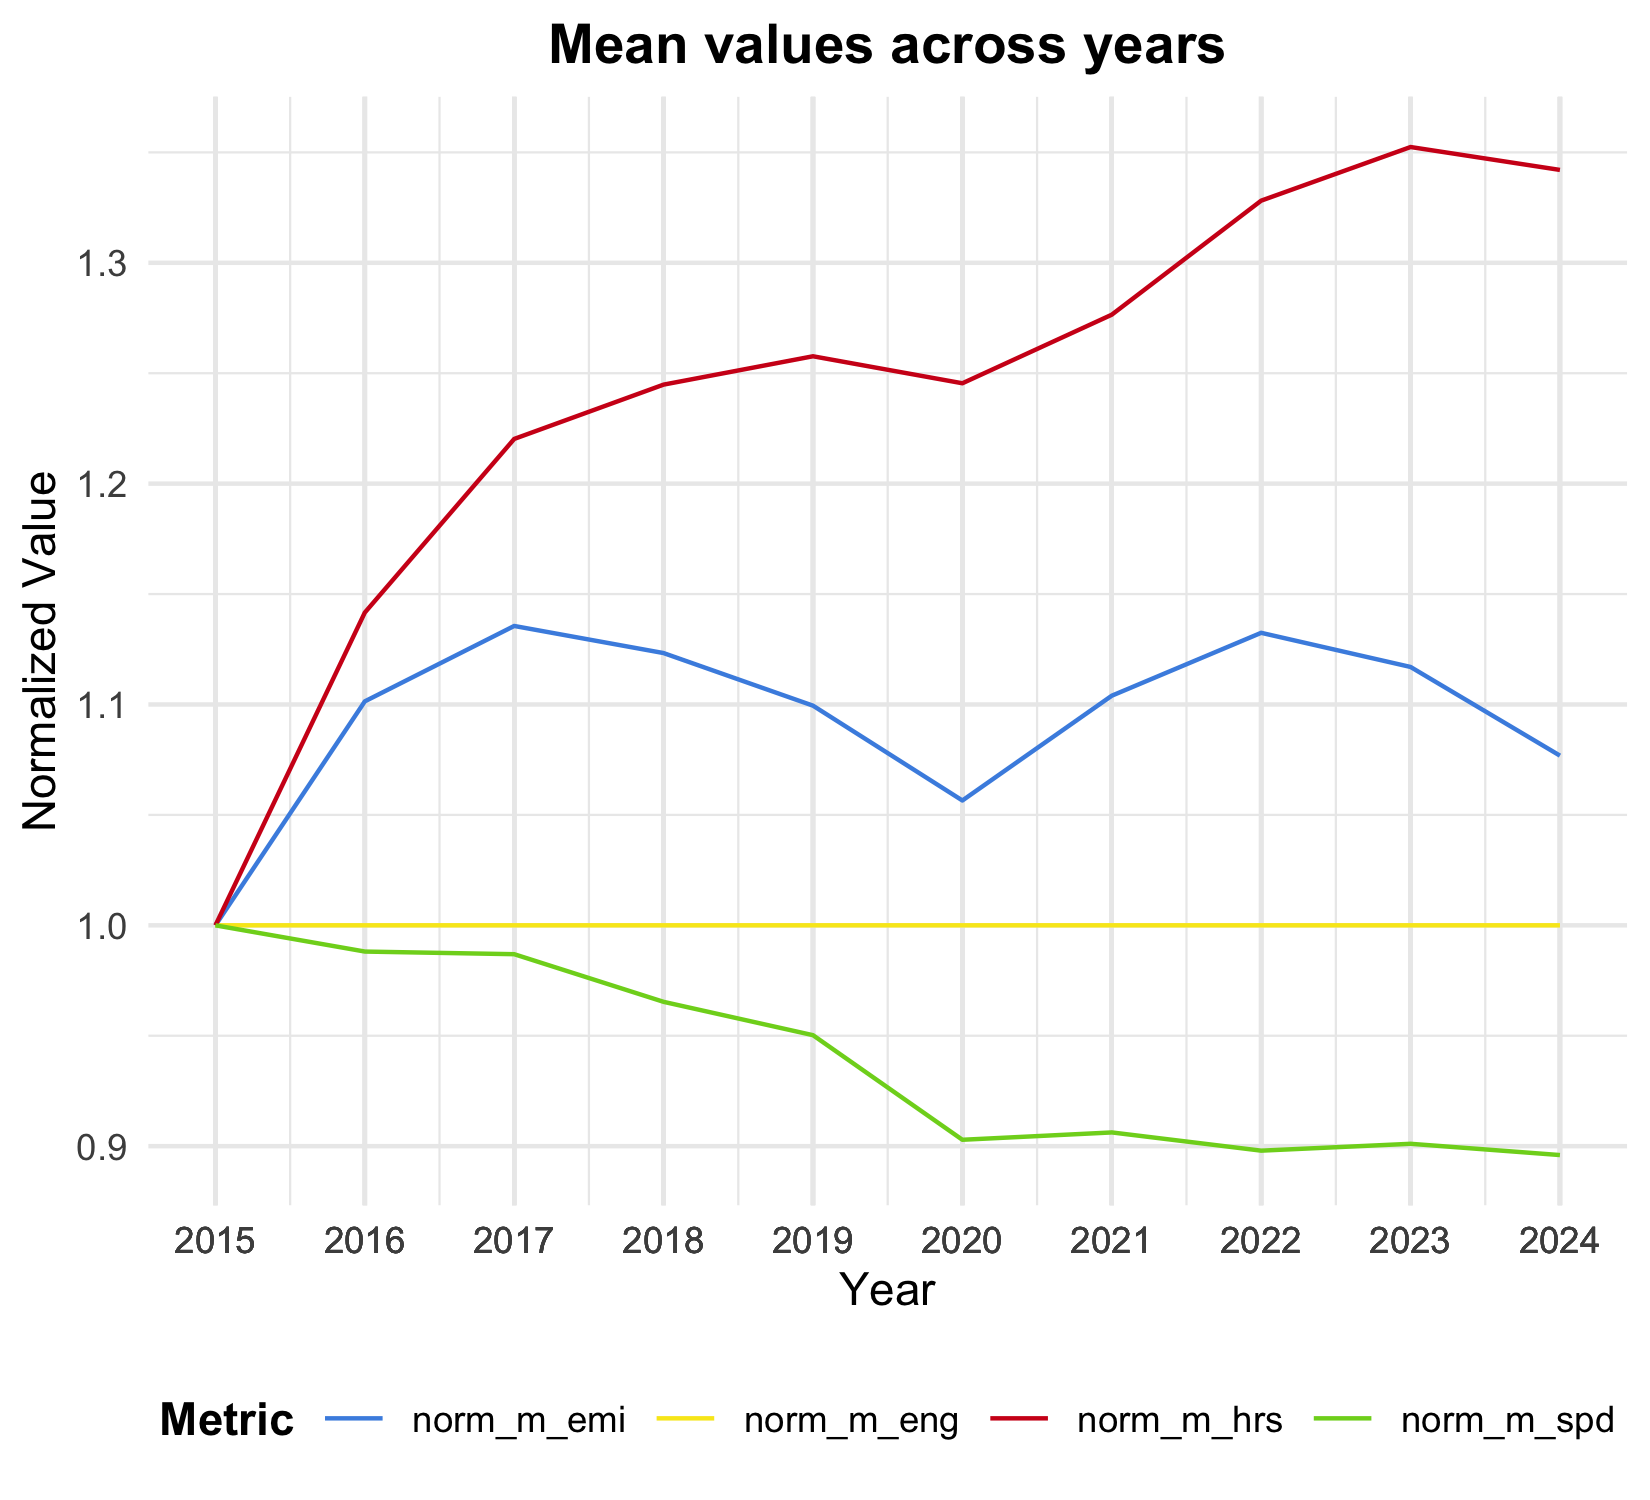
\includegraphics{figures/fig-all-years-operating-vessels-norm-mean-values-from-ping-level-emissions-1.png}

}

\caption{\label{fig-all-years-operating-vessels-norm-mean-values-from-ping-level-emissions}Annual
mean of individual per-vessel CO2 ping emissions (metric tonnes); total
per-vessel operating hours; mean per-vessel main engine power
(killowatts); and mean per-vessel speed (knots) for the set of
AIS-broadcasting operating in all years, where each line is colored by
the last operation year. Values are normalized againts 2015 estimates.}

\end{figure}%

The relationship between hours and speeds may be misleading, as the
dataset includes information from both trips and port stays. While hours
accumulate regardless of whether a vessel is on a trip or at port,
distances covered during port stays are minimal, leading to
misrepresented speed values.

To address this, we can assess the actual changes in these parameters
(considering distances as well) by exclusively analyzing emissions from
trips. Below, we present data extracted from the trip emissions dataset,
aggregated by vessel for all trips starting in a given year. This shows
a completely different trend compared to the observations above.
Restricting vessel information to those that has a registered at least
one trip in each year has moved the number of vessels considered in this
representation from 101754 to 67715

\begin{figure}[H]

\centering{

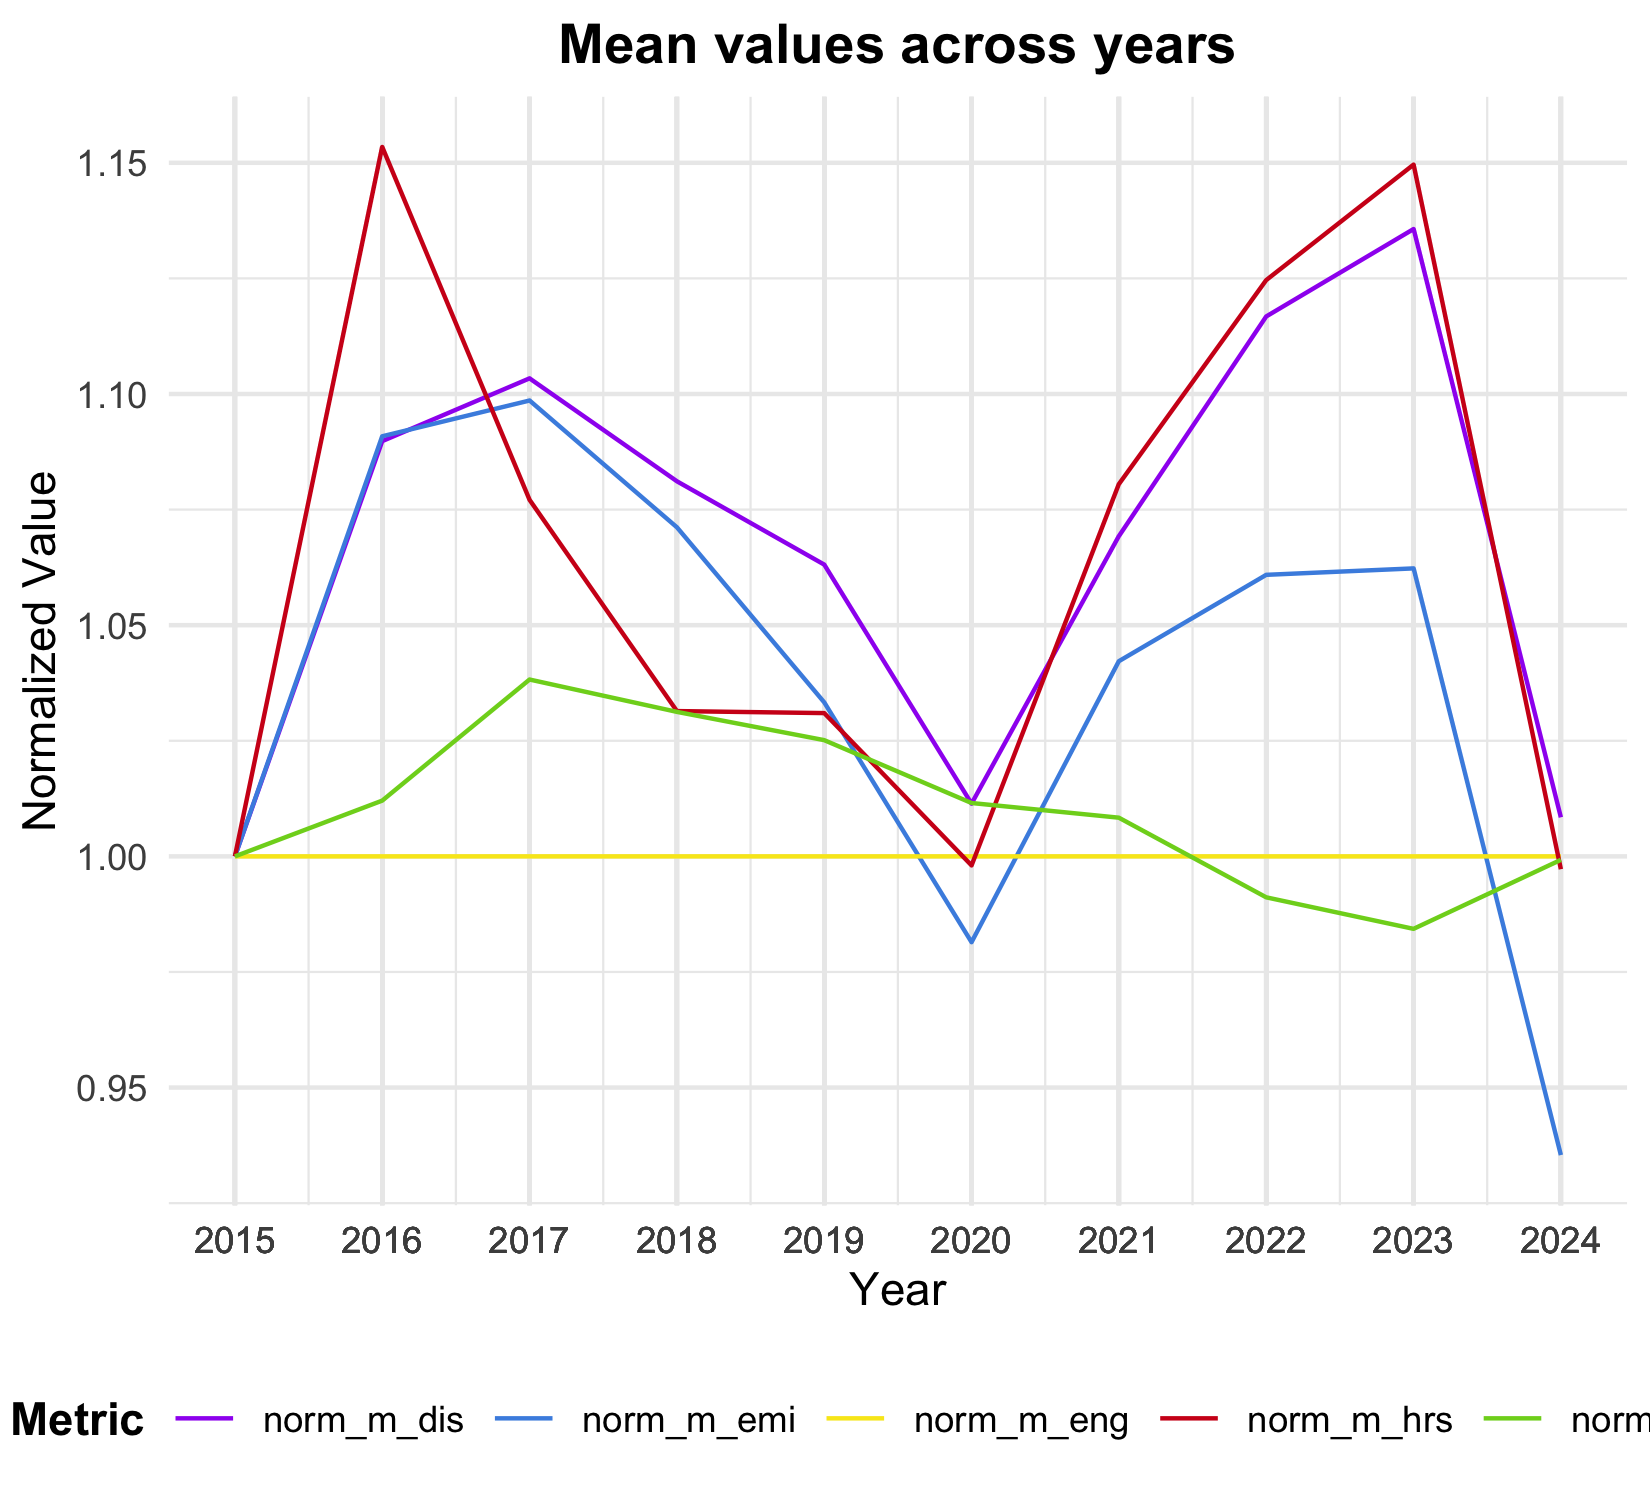
\includegraphics{figures/fig-all-years-operating-vessels-norm-mean-values-from-trip-level-emissions-1.png}

}

\caption{\label{fig-all-years-operating-vessels-norm-mean-values-from-trip-level-emissions}Annual
mean of individual per-vessel CO2 trip emissions (metric tonnes); total
per-vessel operating hours; mean per-vessel main engine power
(killowatts); mean per-vessel speed (knots); and total distance traveled
for the set of AIS-broadcasting operating in all years, where each line
is colored by the last operation year.}

\end{figure}%

\subsection{Assessing number of
vessels}\label{assessing-number-of-vessels}

\subsection{Methods}\label{methods}

\subsubsection{Outside and withing S1 footprint
ratios}\label{outside-and-withing-s1-footprint-ratios}

\begin{figure}[H]

\centering{


\includegraphics{figures/fig-map-dark-to-ais-s1-ratio-1.png}

}

\caption{\label{fig-map-dark-to-ais-s1-ratio}Mean ratio value within and
outside S1 footprint, aggregated across all years, and vessel lengths,
for representation purposes. Model inputs are disaggregated by pixel,
month, vessel class and length bin.}

\end{figure}%

\subsubsection{Fraction of S1-detected
vessels}\label{fraction-of-s1-detected-vessels}

\begin{figure}[H]

\centering{


\includegraphics{figures/fig-dark-vessel-fraction-detected-time-series-1.png}

}

\caption{\label{fig-dark-vessel-fraction-detected-time-series}Fraction
of S1-detected vessels matched AIS-broadcasting vessels over time,
disaggregated by vessel type and length size class}

\end{figure}%

\subsubsection{Summary of global annual CO2 dark emissions over
time}\label{summary-of-global-annual-co2-dark-emissions-over-time}

\begin{figure}[H]

\centering{


\includegraphics{figures/fig-global-annual-co2-dark-emissions-by-type-1.png}

}

\caption{\label{fig-global-annual-co2-dark-emissions-by-type}Summary of
global annual CO2 dark emissions over time, disaggregated by vessel
type.}

\end{figure}%




\end{document}
